%%%%%%%%%%%%%%%%%%%%%%%%%%%%%%%%%%%%%%%%%%%%%%%%%%%%%%%%%%%%%%%%%%%%%%%%%%%%%%%%%%%%%%%%%
% Khóa luận tốt nghiệp/Tiểu luận 
% LaTeX Template
% Phiên bản 1.0 (tạo ra ngày 05/10/2022)
%
% Template này có thể được download tại:
% https://github.com/cpc1996/HUS-Dissertation-Template
%
% Phiên bản 1.0 được chỉnh sửa bởi:
% Công Phương Cao (congphuongcao_t59@hus.edu.vn)
% Nguyễn Cảnh Việt (vietncp@gmail.com)
% Nguyễn Tiến Cường (ngtiencuong@gmail.com)
%
% Template được tham khảo từ một phiên bản template của:
% Steve Gunn (http://users.ecs.soton.ac.uk/srg/softwaretools/document/templates/)
% Sunil Patel (http://www.sunilpatel.co.uk/thesis-template/)
%
%%%%%%%%%%%%%%%%%%%%%%%%%%%%%%%%%%%%%%%%%%%%%%%%%%%%%%%%%%%%%%%%%%%%%%%%%%%%%%%%%%%%%%%%%


%----------------------------------------------------------------------------------------
%	(KHÔNG CHỈNH SỬA PHẦN NÀY)
%
%	PHẦN 1: CÁC PACKAGE CƠ BẢN VÀ CÁC TÙY CHỈNH VĂN BẢN
%----------------------------------------------------------------------------------------

\documentclass[
12pt,
oneside,
english,
doublespacing,
nolistspacing,
liststotoc,
parskip,
headsepline,
chapterinoneline,
]{MastersDoctoralThesis}

% \usepackage[utf8]{inputenc} 
\usepackage[utf8]{vietnam} 
%\usepackage[T1]{fontenc}

\usepackage{mathptmx}
\usepackage{amsmath}
\allowdisplaybreaks

%https://www.overleaf.com/learn/latex/Biblatex_citation_styles
%\usepackage[backend=bibtex,style=authoryear,natbib=true]{biblatex}
\usepackage[backend=bibtex,style=numeric,citestyle=ieee,natbib=true]{biblatex}

\addbibresource{main.bib}

\usepackage[autostyle=true]{csquotes}


%----------------------------------------------------------------------------------------
%	PHẦN 2: CÁC PACKAGE BỔ TRỢ THÊM VÀO TRONG QUÁ TRÌNH BIÊN SOẠN
%----------------------------------------------------------------------------------------

\usepackage{multirow}
\usepackage{subfigure}
\usepackage[fontsize=13pt]{scrextend}

%https://www.sascha-frank.com/latex-font-size.html
%https://tex.stackexchange.com/questions/103286/how-to-change-section-subsection-font-size
\usepackage{titlesec}

\titleformat{\section}
{\normalfont\fontsize{13}{13}\bfseries}{\thesection}{1em}{}

\titleformat{\subsection}
{\normalfont\fontsize{13}{13}\bfseries\itshape}{\thesubsection}{1em}{}

\usepackage{listings} 		% Liệt kê/trích dẫn code

%https://tex.stackexchange.com/questions/351961/how-to-indent-code-in-beginverbatim
\usepackage{fancyvrb} 		% Fancy Verbatim
\fvset{tabsize=4,vspace=0pt,fontsize=\footnotesize}

\usepackage{longtable} 		% Bảng dài - Long table

\usepackage[figuresright]{rotating} % Bảng ngang - Sideways table
\usepackage{tabularx}

\usepackage{fontawesome5} 	% Các biểu tượng, ký hiệu đặc biệt

\usepackage{tikz} 			% Vẽ hình
\usetikzlibrary{calc}


%----------------------------------------------------------------------------------------
%	(KHÔNG CHỈNH SỬA PHẦN NÀY)
%
%	PHẦN 3: CÁC TÙY CHỈNH LIỆT KÊ SOURCE CODE 
%----------------------------------------------------------------------------------------

%https://tex.stackexchange.com/questions/33039/using-ttfamily-with-bfseries-or-how-to-enable-bold-in-fixed-width-font
\renewcommand{\ttdefault}{pcr}
\newenvironment{pcr}{\fontfamily{pcr}\selectfont}

\definecolor{backcolor}{HTML}{f5fffc}
\definecolor{darkpink}{rgb}{0.75,0.25,0.5}
\definecolor{cadetblue}{rgb}{.6,.8,.8}

\lstset{
	tabsize			= 4,
	breaklines		= true,
	basicstyle		= \ttfamily\color{black}\bfseries\scriptsize,
	identifierstyle	= \ttfamily\color{black},
	keywordstyle	= \ttfamily\color{blue}\bfseries,  
	stringstyle		= \ttfamily\color{Red},
	commentstyle	= \itshape\color{cyan},
	%===================================================================================
	frame			= l,
	numbers			= left,
	stepnumber		= 1, 
	upquote			= true,
	numberstyle		= \tiny\color{Gray},
	backgroundcolor	= \color{backcolor},
	rulecolor		= \color{lightgray},
	rulesepcolor	= \color{lightgray},
	showstringspaces=false
	keepspaces		= true, 
	belowcaptionskip= 1\baselineskip,
	xleftmargin		= \parindent,
	%	escapeinside	= {@}{@},
	numbersep		= 7pt
}

\lstdefinestyle{codeC} {
	%https://www.pvv.ntnu.no/~berland/latex/docs/listings.pdf
	%https://www.overleaf.com/learn/latex/Using_colours_in_LaTeX
	language		= [ISO]C++, 
	basicstyle		= \linespread{1.0}\ttfamily\color{black}\bfseries\scriptsize,
	identifierstyle	= \ttfamily\color{black},
	keywordstyle	= \ttfamily\color{blue}\bfseries,  
	stringstyle		= \ttfamily\color{Red},
	commentstyle	= \itshape\color{cyan}, 
	morekeywords	= {FILE},
	%	emphstyle		= \ttfamily\color{red}\bfseries,
	%	emph			= { auto,break,case,char,const,continue,default,do,double,else,enum,extern,float,for,goto,if,int,long,register,return,short,signed,sizeof,static,struct,switch,typedef,union,unsigned,void,volatile,while,FILE},
	%https://tex.stackexchange.com/questions/283170/using-different-colors-for-different-keywords-in-lstlisting
	classoffset		= 1, % starting new class
	otherkeywords	= {\#include},
	morekeywords	= {\#include},
	keywordstyle	= \ttfamily\color{Green}\bfseries,
	morecomment		= [s][\bfseries\color{Orange}]{<a}{>},% a b d e f i l m n q r s t u v
	morecomment		= [s][\bfseries\color{Orange}]{<b}{>},
	morecomment		= [s][\bfseries\color{Orange}]{<d}{>},
	morecomment		= [s][\bfseries\color{Orange}]{<e}{>},
	morecomment		= [s][\bfseries\color{Orange}]{<f}{>},
	morecomment		= [s][\bfseries\color{Orange}]{<i}{>},
	morecomment		= [s][\bfseries\color{Orange}]{<l}{>},
	morecomment		= [s][\bfseries\color{Orange}]{<m}{>},
	morecomment		= [s][\bfseries\color{Orange}]{<n}{>},
	morecomment		= [s][\bfseries\color{Orange}]{<q}{>},
	morecomment		= [s][\bfseries\color{Orange}]{<r}{>},
	morecomment		= [s][\bfseries\color{Orange}]{<s}{>},
	morecomment		= [s][\bfseries\color{Orange}]{<t}{>},
	morecomment		= [s][\bfseries\color{Orange}]{<u}{>},
	morecomment		= [s][\bfseries\color{Orange}]{<v}{>},
	morecomment		= [l][\bfseries\color{Green}]{\#define},
	classoffset		= 0,
}

\lstdefinestyle{plaintext} {
	%https://www.pvv.ntnu.no/~berland/latex/docs/listings.pdf
	%https://www.overleaf.com/learn/latex/Using_colours_in_LaTeX
	language		= bash, 
	basicstyle		= \linespread{1.0}\ttfamily\color{black}\bfseries\scriptsize,
	identifierstyle	= \ttfamily\color{black},
	keywordstyle	= \ttfamily\color{black}\bfseries,  
	stringstyle		= \ttfamily\color{black},
	commentstyle	= \itshape\color{gray}, 
	%	showspaces		= true,
	%	showstringspaces= true,
	showtabs		= true,
	tab				= \textcolor{lightgray}{$\to$},
%	literate=*
%	{0}{{{\color{darkpink}0}}}{1}
}

\lstdefinestyle{codeMatlab} {
	language		= Matlab,
	basicstyle		= \linespread{1.0}\ttfamily\color{black}\bfseries\scriptsize,
	identifierstyle	= \ttfamily\color{black},
	keywordstyle	= \ttfamily\color{blue}\bfseries,  
	stringstyle		= \ttfamily\color{magenta},
	commentstyle	= \itshape\color{LimeGreen},
	morecomment		= [l][\bfseries\color{red}]{\%\%},
	morekeywords	= {syms,switch,case,otherwise,ones,class,inline,vectorize,factorial,xlim,ylim,ezplot,pie,ezmesh,ezsurf,ezcontour,ezplot3,solve,double,subs,fsolve,fminsearch,compose,jacobian,int,dblquad,triplequad,limit,finverse,simplify,taylor,symsum,evalin,symengine,matlabFunction,poly2sym,lsqcurvefit,ppval,dsolve},
	literate		=*,
	literate		=*
	{^}{\textasciicircum}{1}
}

\lstdefinestyle{codePython} {
	language		= Python,
	basicstyle		= \linespread{1.0}\ttfamily\color{black}\bfseries\scriptsize,
	identifierstyle	= \ttfamily\color{black},
	keywordstyle	= \ttfamily\color{blue}\bfseries,  
	stringstyle		= \ttfamily\color{LimeGreen},
	commentstyle	= \itshape\color{cadetblue},
	morekeywords	= {self},
	emph			={MyClass,__init__},
	emphstyle		=\ttb\color{red},
	literate		=*,
	literate		=*
	{^}{\textasciicircum}{1}
}

%https://www.alanshawn.com/tech/2019/09/01/emulate-terminal.html
\definecolor{tergreen}{rgb}{0,0.6,0}
\definecolor{tergray}{rgb}{0.5,0.5,0.5}
\definecolor{termauve}{rgb}{0.58,0,0.82}
\definecolor{terminalbgcolor}{HTML}{330033}
\definecolor{terminalrulecolor}{HTML}{000099}
\lstdefinestyle{console} {
	backgroundcolor	= \color{terminalbgcolor},
	basicstyle		= \linespread{1.0}\ttfamily\color{white}\bfseries\scriptsize,
	identifierstyle	= \ttfamily\color{white}\bfseries\scriptsize,
	breakatwhitespace=false,
	breaklines		= true,
	captionpos		= b,
	commentstyle	= \color{tergreen},
	deletekeywords	= {...},
	escapeinside	= {\%*}{*)},
	extendedchars	= true,
	frame			= single,
	keepspaces		= true,
	keywordstyle	= \color{blue},
	language		= {},
	morekeywords	= {*,...},
	numbers			= none,
	numbersep		= 5pt,
	framerule		= 2pt,
	numberstyle		= \color{tergray}\tiny\selectfont,
	rulecolor		= \color{terminalrulecolor},
	showspaces		= false,
	showstringspaces= false,
	showtabs		= false,
	stepnumber		= 2,
	stringstyle		= \color{termauve},
	tabsize			= 2,
	literate		=*
}


%----------------------------------------------------------------------------------------
%	(KHÔNG CHỈNH SỬA PHẦN NÀY)
%
%	PHẦN 4: CÁC TÙY CHỈNH KHỔ GIẤY VÀ CĂN LỀ
%----------------------------------------------------------------------------------------

\geometry{
	paper=a4paper,
	inner=3cm,
	outer=2cm,
	bindingoffset=0cm,
	top=0.6cm,
	bottom=2.0cm,
}


%----------------------------------------------------------------------------------------
%	PHẦN 5: THÔNG TIN VỀ Khóa luận tốt nghiệp/Tiểu luận (THESIS INFORMATION)
%----------------------------------------------------------------------------------------

\author{Tên sinh viên thực hiện} 			% Ví dụ: "Nguyễn Thị Thu Thảo"
\thesistitle{Tên của Khóa luận tốt nghiệp/Tiểu luận} % Ví dụ: "Nghiên cứu chế tạo và tính chất quang học của vật liệu nano LaF3:Sm3+"

\supervisor {Tên giảng viên hướng dẫn 1} 	% Ví dụ: "PGS. TS. Nguyễn Ngọc Long"
\supervisorr{Tên giảng viên hướng dẫn 2} 	% Tên này nếu không có thì để trống!

\field{Tên ngành đào tạo} 					% Ví dụ: "Ngành Vật lý", "Ngành Hóa học", v.v.
\program{Tên chương trình đào tạo} 			% Ví dụ: "Chương trình đào tạo chuẩn", "Chương trình đào tạo cử nhân tài năng", v.v.
\doctype{Khóa luận tốt nghiệp đại học hệ chính quy} % Điền vào đây: "Khóa luận tốt nghiệp đại học hệ chính quy" hoặc "Tiểu luận"

\university{\href{http://hus.vnu.edu.vn}{Trường Đại học Khoa học Tự nhiên}}
\department{\href{http://hus.vnu.edu.vn/gioi-thieu/co-cau-to-chuc/khoa-truc-thuoc/khoa-vat-ly.html}{Khoa Vật lý}}

\AtBeginDocument{
	\hypersetup{pdftitle=\ttitle}
	\hypersetup{pdfauthor=\authorname}
}


\begin{document}

\lstset{style=codeC}	% Thiết lập ngôn ngữ C/C++ là ngôn ngữ mặc định cho phần liệt kê souce code của cả bài

\frontmatter 			% Sử dụng hệ thống đánh số La Mã (i, ii, iii, iv...) cho những trang trước phần mục lục

\pagestyle{plain} 


%----------------------------------------------------------------------------------------
%	(KHÔNG CHỈNH SỬA PHẦN NÀY)
%
%	Phần 6: TRANG TIÊU ĐỀ/TRANG BÌA (TITLE PAGE)
%----------------------------------------------------------------------------------------

% TRANG BÌA:
\begin{titlepage}
	\begin{tikzpicture}[overlay,remember picture]
		\draw [line width=3pt]
		($ (current page.north west) + (2.0cm,-2.0cm) $)
		rectangle
		($ (current page.south east) + (-1.5cm,1.8cm) $);
		\draw [line width=1pt]
		($ (current page.north west) + (2.15cm,-2.15cm) $)
		rectangle
		($ (current page.south east) + (-1.65cm,1.95cm) $); 
	\end{tikzpicture}
	\begin{center}
		
		\vspace{-.04\textheight}
		\noindent\scshape
		\large \, \href{https://www.vnu.edu.vn/home/}{ĐẠI HỌC QUỐC GIA HÀ NỘI}\\
		\vspace{-0.25cm}{\large \MakeUppercase \univname}\\
		\vspace{-0.25cm}{\large \bfseries \MakeUppercase \deptname}\\[0.5cm]
		
\includegraphics{Logo/Logo_HUS_notext_nocolor}
		
		\vspace{1.0cm}
		
		{\large \MakeUppercase \authorname}
		
		\vspace{2.5cm}
		
		{\Large \bfseries \MakeUppercase\ttitle\par}
		
		\vspace{2.5cm}
		
		{\normalsize \docname\\ \fieldname\\ (\progname)\\}
	
		\vfill
		
		\textbf{Hà Nội - \the\year{}}
	\end{center}
\end{titlepage}


% TRANG BÌA LÓT:
\begin{titlepage}
	\begin{tikzpicture}[overlay,remember picture]
		\draw [line width=3pt]
		($ (current page.north west) + (2.0cm,-2.0cm) $)
		rectangle
		($ (current page.south east) + (-1.5cm,1.8cm) $);
		\draw [line width=1pt]
		($ (current page.north west) + (2.15cm,-2.15cm) $)
		rectangle
		($ (current page.south east) + (-1.65cm,1.95cm) $); 
	\end{tikzpicture}
	\begin{center}
		
		\vspace{-.04\textheight}
		\noindent\scshape
		\large \, \href{https://www.vnu.edu.vn/home/}{ĐẠI HỌC QUỐC GIA HÀ NỘI}\\
		\vspace{-0.25cm}{\large \MakeUppercase \univname}\\
		\vspace{-0.25cm}{\large \bfseries \MakeUppercase \deptname}\\[0.5cm]
		
\includegraphics{Logo/Logo_HUS_notext}
		
		\vspace{1.0cm}
		
		{\large \MakeUppercase \authorname}
		
		\vspace{2.5cm}
		
		{\Large \bfseries \MakeUppercase\ttitle\par}
		
		\vspace{2.5cm}
		
		{\normalsize \docname\\ \fieldname\\ (\progname)\\}
	 
	 	\vspace{2.5cm}
	 	
		\begin{minipage}[t]{0.49\textwidth}
			\begin{flushright} \large \bfseries
				Giảng viên hướng dẫn:\;
			\end{flushright}
		\end{minipage}
		\begin{minipage}[t]{0.5\textwidth}
			\begin{flushleft} \large \bfseries
				\supname\\
				\supnamee
			\end{flushleft}
		\end{minipage}
	
		\vfill
		
		\textbf{Hà Nội - \the\year{}}
	\end{center}
\end{titlepage}


%----------------------------------------------------------------------------------------
%	Phần 7: DANH NGÔN (QUOTES)
%----------------------------------------------------------------------------------------

\vspace*{0.2\textheight}

\noindent\enquote{\itshape 
	Cái tôi và sự hiểu biết tỷ lệ nghịch với nhau. Hiểu biết càng nhiều cái tôi càng bé. Hiểu biết càng ít, cái tôi càng to.
}\bigbreak

\hfill Albert Einstein


%----------------------------------------------------------------------------------------
%	Phần 8: LỜI CẢM ƠN (ACKNOWLEDGEMENTS)
%----------------------------------------------------------------------------------------

\begin{acknowledgements}
	\addchaptertocentry{\acknowledgementname}
	\thispagestyle{empty}
	Sự ghi nhận và lời cảm ơn đối đối với những người liên quan, đừng quên cảm ơn giảng viên hướng dẫn của bạn\ldots
\end{acknowledgements}


%----------------------------------------------------------------------------------------
%	(KHÔNG CHỈNH SỬA PHẦN NÀY)
%
%	Phần 9: MỤC LỤC (LIST OF CONTENTS/FIGURES/TABLES PAGES)
%----------------------------------------------------------------------------------------

\begin{spacing}{1.15}
	\tableofcontents 	% In ra mục lục chính
\end{spacing}

\begin{spacing}{1.15}
	\listoffigures 		% In ra danh sách hình vẽ
\end{spacing}

\begin{spacing}{1.15}
	\listoftables		% In ra danh sách bảng
\end{spacing}


%----------------------------------------------------------------------------------------
%	Phần 10: DANH SÁCH TÊN VIẾT TẮT (ABBREVIATIONS)
%----------------------------------------------------------------------------------------

\begin{abbreviations}{ll} % Thêm danh sách tên viết tắt (dưới dạng một bảng có 2 cột)

\textbf{TVT} & \textbf{T}ên \textbf{V}iết \textbf{T}ắt\\
\textbf{ĐTĐ} & \textbf{Đ}ặt (nó) \textbf{T}ại \textbf{Đ}ây\\

\end{abbreviations}


%----------------------------------------------------------------------------------------
%	Phần 11: CÁC HẰNG SỐ VẬT LÝ/THÔNG SỐ KĨ THUẬT (PHYSICAL CONSTANTS/OTHER DEFINITIONS)
%----------------------------------------------------------------------------------------

\begin{constants}{lr@{${}={}$}l} % Thêm danh sách các hằng số (dưới dạng một bảng có 3 cột)

%	Lệnh \SI{}{} được cung cấp bởi gói siunitx, hãy đọc tài liệu hướng dẫn để biết cách sử dụng nó

%	Tên hằng số 	 & $Biểu tượng$	& $Hằng số$ cùng với đơn vị\\
	Vận tốc ánh sáng & $c_{0}$		& \SI{2.99792458e8}{\meter\per\second} (chính xác)\\

\end{constants}


%----------------------------------------------------------------------------------------
%	Phần 12: DANH SÁCH KÝ HIỆU (SYMBOLS)
%----------------------------------------------------------------------------------------

\begin{symbols}{lll} % Thêm danh sách các ký hiệu (dưới dạng một bảng có 3 cột)

%   Ký hiệu	& Ý nghĩa		& Đơn vị \\
	$a$		& khoảng cách	& \si{\meter} \\
	$P$		& công suất		& \si{\watt} (\si{\joule\per\second}) \\

	\addlinespace % Khoảng cách để phân biệt giữa ký hiệu Latin với ký hiệu La Mã

	$\omega$ & tần số góc	& \si{\radian} \\

\end{symbols}


%----------------------------------------------------------------------------------------
%	(KHÔNG CHỈNH SỬA PHẦN NÀY)
%
%	Phần 13: LỜI ĐỀ TẶNG (DEDICATION)
%----------------------------------------------------------------------------------------

%\dedicatory{Dành tặng/Dành cho/Gửi tới\ldots} 


%----------------------------------------------------------------------------------------
%	Phần 14: NỘI DUNG/CÁC CHƯƠNG Khóa luận tốt nghiệp/Tiểu luận (THESIS CONTENT - CHAPTERS)
%----------------------------------------------------------------------------------------

\mainmatter % Bắt đầu đánh số trang (1,2,3...)

\pagestyle{plain}

% Hãy thêm những chương (chapter) của khóa luận/tiểu luận vào thư mục Chapters
% Hãy bỏ chú thích những dòng nếu bạn đã bổ sung những chương vào

% Chương 1

\chapter{MỞ ĐẦU - GIỚI THIỆU CHUNG} % Tên của chương

\label{Chapter1} % Để trích dẫn chương này ở chỗ nào đó trong bài, hãy sử dụng lệnh \ref{Chapter1} 

%----------------------------------------------------------------------------------------

% Định nghĩa một số lệnh cần thiết để điều chỉnh định dạng cho một số nội dung nhất định trong bài
\newcommand{\keyword}[1]{\textbf{#1}}
\newcommand{\tabhead}[1]{\textbf{#1}}
\newcommand{\code}[1]{\texttt{#1}}
\newcommand{\file}[1]{\texttt{\bfseries#1}}
\newcommand{\option}[1]{\texttt{\itshape#1}}

%----------------------------------------------------------------------------------------

\section{Lời mở đầu}

Chào mừng bạn đến với template \LaTeX{} khóa luận tốt nghiệp/tiểu luận của Bộ môn Tin học Vật lý. Đây là một template đẹp và dễ sử dụng cho việc biên soạn khóa luận tốt nghiệp/tiểu luận sử dụng hệ thống gõ \LaTeX{}.

Nếu bạn đang hoặc sẽ biên soạn khóa luận tốt nghiệp/tiểu luận và chủ đề liên quan đến kĩ thuật hoặc toán học thì việc biên soạn trên \LaTeX{} là rất đáng cân nhắc vì đây là cách giúp bạn có thể ngồi xuống và tập trung vào nội dung viết cốt lõi mà không cần lo lắng về mặt định dạng (format) cũng như lãng phí thời gian vào việc tinh chỉnh phần mềm soạn thảo văn bản.

\LaTeX{} có thể dễ dàng biên soạn các tài liệu một cách chuyên nghiệp mà lên tới hàng trăm hoặc hàng nghìn trang. Với câu lệnh đơn giản, nó tự động sắp đặt mục lục, lề, tiêu đề/chân trang, và giữ cho định dạng thống nhất và đẹp đẽ. Một trong những thế mạnh chính của \LaTeX{} là việc gõ các công thức toán học, thậm chí các công thức \emph{rất phức tạp}. Ngay cả khi những phương trình này là những vấn đề phức tạp và khó khăn nhất mà chỉ có thể được giải được bằng siêu máy tính, bạn có thể yên tâm là ít nhất \LaTeX{} sẽ làm cho chúng trông \emph{lộng lẫy}.


%----------------------------------------------------------------------------------------

\section{Học \LaTeX{}}

\LaTeX{} không phải một chương trình \textsc{wysiwyg} (What You See is What You Get, tạm dịch: \textit{Giao diện tương tác tức thời - mắt thấy tay làm}), không giống các trình soạn thảo văn bản như Microsoft Word hoặc Pages của Apple. Một văn bản được viết cho \LaTeX{} chỉ đơn thuần là một file (tập tin) văn bản đơn giản \emph{không có định dạng}. Bạn nói với \LaTeX{} cách bạn muốn văn bản định dạng bằng cách viết những dòng lệnh đơn giản trong văn bản, ví dụ, nếu bạn muốn sử dụng \emph{chữ in nghiêng (italic)}, bạn viết lệnh \verb|\emph{nội dung}| và đưa nội dung bạn muốn in nghiêng vào trong dấu ngoặc nhọn. Điều này có nghĩa rằng \LaTeX{} là một ngôn ngữ lập trình \enquote{đánh dấu (mark-up)}, tương tự như HTML.


\subsection{Một tài liệu ngắn gọn giới thiệu về \LaTeX{}}

Nếu bạn mới tiếp cận với \LaTeX{} thì có một cuốn sách rất đáng tham khảo -- file PDF miễn phí có sẵn trên mạng -- tên là, \enquote{The Not So Short Introduction to \LaTeX{}}. Tiêu đề cuốn sách được rút gọn thành chỉ còn \emph{lshort}. Bạn có thể download bản mới nhất tại đây:
\url{http://www.ctan.org/tex-archive/info/lshort/english/lshort.pdf}

Cuốn sách được viết bằng một số ngôn ngữ. Trong đó bản tiếng Việt tại đây:
\url{https://mirror.kku.ac.th/CTAN/info/lshort/vietnamese/lshort-vi.pdf}

Bạn nên dành ra một chút thời gian để học cách sử dụng \LaTeX{} bằng cách tạo một vài văn bản `test' nho nhỏ, hoặc ngó qua một vài templates tại:\\
\url{http://www.LaTeXTemplates.com}\\
Bỏ ra một chút công sức ngay lúc này giúp bạn sẽ không phải chật vật học một hệ thống khi những gì bạn thực sự cần làm là tập trung viết nội dung.


\subsection{Hướng dẫn ngắn về công thức toán học trong \LaTeX{}}

Nếu bạn đang biên soạn khóa luận tốt nghiệp/tiểu luận có chủ đề liên quan đến kĩ thuật hoặc toán học thì có thể bạn sẽ muốn đọc tài liệu bới AMS (American Mathematical Society, tạm dịch: Hiệp hội toán học Mĩ), \enquote{A Short Math Guide for \LaTeX{}}. Bạn có thể download tại đây:
\url{http://www.ams.org/tex/amslatex.html}
dưới mục \enquote{Additional Documentation} ở cuối trang web, phần \enquote{Short Math Guide for \LaTeX{}}.


\subsection{Các ký hiệu toán học phổ biến trong \LaTeX{}}

Có vô số các ký hiệu toán học có sẵn trên \LaTeX{} và bạn sẽ phải nỗ lực rất nhiều để tìm hiểu tất cả các lệnh cho chúng. Thay vào đó, bạn có thể tra cứu những ký hiệu toán học phổ biến nhất tại đây:\\
\url{http://www.sunilpatel.co.uk/latex-type/latex-math-symbols/}

Bạn có thể sử dụng trang này như một bảng tra cứu. Những ký hiệu được làm to, hình ảnh sắc nét nên bạn có thể nhanh chóng tìm thấy câu lệnh \LaTeX{} cho ký hiệu cần dùng.


\subsection{\LaTeX{} trên máy tính Mac}

Bản phân phối \LaTeX{} có sẵn cho nhiều hệ thống bao gồm Windows, Linux và Mac OS X. Gói dành cho OS X được gọi là MacTeX và nó chứa tất cả các ứng dụng bạn cần -- được đóng gói cùng nhau và tùy chỉnh trước -- cho một môi trường \LaTeX{} và luồng công việc hoạt động đầy đủ.

MacTeX bao gồm một trình soạn thảo \LaTeX{} chuyên dụng tùy chỉnh được gọi là TeXShop để viết các file `\file{.tex}' của bạn và BibDesk: một chương trình để quản lý các tài liệu tham khảo và tạo phần danh mục trích dẫn của bạn dễ dàng như quản lý bài hát và tạo danh sách phát trong iTunes.


\subsection{\LaTeX{} trên Linux}
Đối với máy tính sử dụng hệ điều hành Linux, gói phổ biến dành cho hệ điều hành này là \code{texlive} (dành cho Debian hoặc Ubuntu) và \code{tetex} (dành cho RedHat hoặc CentOS). Tương tự như trình biên dịch \code{gcc} cho ngôn ngữ lập trình C, \code{texlive} và \code{tetex} là một trình biên dịch đóng vai trò biên dịch \LaTeX{}. Bạn hoàn toàn có thể dùng bất kì trình soạn thảo nào có sẵn trên máy để biên soạn \LaTeX{} tuy nhiên một trình soạn thảo \LaTeX{} chuyên dụng (chẳng hạn như \href{https://www.texstudio.org}{\code{texstudio}}) sẽ giúp bạn tiết kiệm phần lớn thời gian và công sức.


%----------------------------------------------------------------------------------------

\section{Bắt đầu với template này}

Nếu bạn đã quen thuộc với \LaTeX{} thì bạn nên tìm hiểu cấu trúc thư mục của template và sau đó thay thế thông tin cá nhân của mình trong phần \emph{THÔNG TIN VỀ Khóa luận tốt nghiệp/Tiểu luận} trong file \file{main.tex}. Bạn có thể chỉnh sửa phần còn lại của file này tùy theo bậc học/trường đại học của bạn. Mục \ref{FillingFile} ở trang \pageref{FillingFile} sẽ giúp bạn làm điều này. Hãy đảm bảo rằng bạn đọc mục \ref{ThesisConventions} về quy định của khóa luận để có thể sử dụng template này một cách tốt nhất.

Nếu bạn mới tiếp cận với \LaTeX{} thì bạn nên đọc hết phần thông tin còn lại trong tài liệu này.

Trước khi bạn bắt đầu sử dụng template này, bạn nên đảm bảo rằng định dạng của template tuân theo quy định về định dạng của khóa luận tốt nghiệp do trường bạn đề ra. Trong hầu hết các trường hợp, định dạng và bố cục của template này sẽ phù hợp. Nếu không, template có thể chỉ cần một số thay đổi nhỏ để khiến định dạng template khớp với định dạng do trường bạn đề ra. Những thay đổi này sẽ cần được thực hiện ở file \file{MastersDoctoralThesis.cls}.


\subsection{Thông tin về template này}

Template \LaTeX{} này được tạo ra dựa trên file định dạng \LaTeX{} của Steve R. Gunn thuộc Đại học Southampton (Vương quốc Anh), khoa Điện tử và Khoa học Máy tính. Bạn có thể tham khảo file định dạng gốc tại trang:
\url{http://www.ecs.soton.ac.uk/~srg/softwaretools/document/templates/}

File \file{ecsthesis.cls} của Steve sau đó được điều chỉnh bởi Sunil Patel bằng cách bổ sung khung và cấu trúc thư mục để chia nhỏ và sắp đặt các file nội dung. Template thu được có thể tìm thấy tại trang:\\
\url{http://www.sunilpatel.co.uk/thesis-template}

Template của Sunil được cung cấp miễn phí tại \url{http://www.LaTeXTemplates.com} nơi mà nó được chỉnh sử nhiều lần nữa dựa trên ý kiến phản hồi và câu hỏi của người dùng. Phiên bản 2.0 trở đi của template được cải tiến nhiều đến mức ta khó lòng có thể nhận ra so với bản đầu tiên. Công việc tạo ra phiên bản 2.0 được thực hiện bởi \href{mailto:vel@latextemplates.com}{Vel} và Johannes Böttcher.

Ngoài ra, phiên bản tiếng Việt mà các bạn đang thấy ở đây được thực hiện bởi các thành viên của Bộ môn Tin học Vật lý, trường ĐHKHTN--ĐHQGHN. Mọi ý kiến góp ý hoặc câu hỏi, các bạn có thể gửi mail cho thầy \href{mailto:vietncp@gmail.com }{Cảnh Việt} và \href{mailto:ngtiencuong@gmail.com }{Tiến Cường}.


%----------------------------------------------------------------------------------------

\section{Những thứ mà template này bao gồm}

\subsection{Các thư mục (Folder)}

Template này ban đầu có định dạng file \file{zip}, sau đó có thể giải nén thành các file và thư mục. Các tên của thư mục hầu như phản ảnh đúng nội dung bên trong:

\keyword{Appendices} (phụ lục) -- thư mục này là nơi bạn đưa phần nội dung phụ lục vào. Mỗi mục của phụ lục nên được lưu lại thành một file \file{.tex} riêng. Một ví dụ và một template phụ lục đã được để sẵn trong thư mục này.

\keyword{Chapters} -- (chương) thư mục này là nơi bạn lưu nội dung các chương (chapter) của khóa luận tốt nghiệp/tiểu luận. Một khóa luận/tiểu luận thường có khoảng 5 chương, tùy thuộc vào quy định cụ thể của khóa luận/tiểu luận cũng như tùy thuộc vào từng cơ sở đào tạo. Mỗi chương nên được lưu lại thành một file \file{.tex} riêng. Các chương có thể được phân chia như sau (ví dụ):
\begin{itemize}
	\item Mở đầu/Lời mở đầu (tùy chọn)
	\item Chương 1: Giới thiệu về nội dung khóa luận tốt nghiệp/tiểu luận
	\item Chương 2: Kiến thức nền tảng và các nguyên lý
	\item Chương 3: Sắp đặt thí nghiệm (Phòng thí nghiệm)
	\item Chương 4: Chi tiết thí nghiệm 1
	\item Chương 5: Chi tiết thí nghiệm 2
	\item Chương 6: Thảo luận về các kết quả thí nghiệm
	\item Chương 7: Kết luận và định hướng nghiên cứu trong tương lai
\end{itemize}

Bố cục chương như trên chuyên dành cho các ngành khoa học thực nghiệm, chuyên ngành của bạn có thể khác.

\keyword{Figures} (hình vẽ) -- thư mục này chứa tất cả hình vẽ có trong khóa luận/tiểu luận. Chúng là những hình vẽ cuối cùng sẽ xuất hiện ở trong văn bản khóa luận/tiểu luận.


\subsection{Các tập tin (file)}

Một số file cũng được bao gồm vào trong template. Hầu hết số trong số chúng là những file văn bản không định dạng và bạn có thể thấy nội dung thông qua một trình soạn thảo văn bản bất kì. Sau khi biên dịch xong, bạn sẽ thấy nhiều hơn các file phụ trợ (auxiliary file) được tạo ra bởi \LaTeX{} hoặc BibTeX và những file mà bạn không cần phải xóa hay quan tâm:

\keyword{main.bib} -- đây là một file quan trọng chứa tất cả các thông tin danh mục trích dẫn và tài liệu tham khảo mà bạn sẽ trích dẫn trong khóa luận/tiểu luận (sử dụng BibTeX). Bạn có thể viết nó một cách thủ công, nhưng có các phần mềm quản lý trích dẫn sẽ giúp bạn tạo và quản lý. Tài liệu tham khảo (bibliography) là một mục lớn trong \LaTeX{} và bạn có lẽ sẽ cần đọc về định dạng BibTeX trước khi bắt đầu biên soạn. Các phần mềm quản lý trích dẫn hiện nay cho phép bạn trích xuất các trích dẫn theo định dạng BibTeX, thứ sẽ tiết kiệm công sức của các bạn rất nhiều.

\keyword{MastersDoctoralThesis.cls} -- đây là một file quan trọng. Nó là file chứa các cài đặt định dạng \LaTeX{} của khóa luận tốt nghiệp/tiểu luận.

\keyword{setspace.sty} -- đây là một file quan trọng. Nó chứa các cài đặt về căn chỉnh các khoảng cách như lề, dòng, khổ của khóa luận tốt nghiệp/tiểu luận được đọc bởi file \file{MastersDoctoralThesis.cls}.

\keyword{setlst.sty} -- đây là một file quan trọng. Nó chứa các cài đặt về liệt kê/trích dẫn code của khóa luận tốt nghiệp/tiểu luận được đọc bởi file \file{main.tex}.

\keyword{main.pdf} -- đây là file khóa luận/tiểu luận đẹp đẽ (dưới định dạng file PDF) tạo ra bởi \LaTeX{}. Trong template này, file PDF được cung cấp sẵn. Sau khi bạn biên dịch lại template, bạn sẽ nhận được một file PDF y hệt.

\keyword{main.tex} -- đây là một file quan trọng. Đây là file sẽ được \LaTeX{} biên dịch để tạo ra khóa luận/tiểu luận của bạn dưới định dạng file PDF. Nó chứa các khung và cấu trúc nội dung mà nói cho \LaTeX{} biết cách bố trí bố cục của khóa luận/tiểu luận. File này được ghi chú (comment) rất chi tiết nên bạn có thể biết chính xác thứ mỗi dòng code thực hiện và tại sao chúng ở đó. Sau khi bạn thêm thông tin cá nhân vào phần \emph{THÔNG TIN VỀ Khóa luận tốt nghiệp/Tiểu luận} -- bạn bây giờ đã bắt đầu biên soạn khóa luận/tiểu luận của mình!

\keyword{main-cover.tex} -- đây là một file quan trọng. Nó chứa các đoạn code mô tả bìa chính (main cover) của khóa luận tốt nghiệp/tiểu luận được đọc bởi file \file{main.tex}.

\keyword{sub-cover.tex} -- đây là một file quan trọng. Nó chứa các đoạn code mô tả bìa phụ (sub-cover) của khóa luận tốt nghiệp/tiểu luận được đọc bởi file \file{main.tex}.

Những file mà không có sẵn trong template mà được tạo ra bởi \LaTeX{} như những file phụ trợ, bao gồm:

\keyword{main.aux} -- đây là một file phụ trợ được tạo ra bởi \LaTeX{}, nếu như bị xóa thì \LaTeX{} sẽ đơn thuần tạo lại nó khi bạn biên dịch lại file \file{main.tex}.

\keyword{main.bbl} -- đây là một file phụ trợ được tạo ra bởi BibTeX, nếu như bị xóa thì BibTeX sẽ đơn thuần tạo lại nó khi bạn chạy file \file{main.aux}. Trong khi file \file{.bib} chứa tất cả các trích dẫn bạn có, thì file \file{.bbl} chứa các trích dẫn bạn thực tế trích dẫn trong khóa luận/tiểu luận và nó được sử dụng để tạo nên mục tài liệu tham khảo ở cuối khóa luận/tiểu luận.

\keyword{main.blg} -- đây là một file phụ trợ được tạo ra bởi BibTeX, nếu như bị xóa thì BibTeX sẽ đơn thuần tạo lại nó khi bạn chạy file \file{main.aux}.

\keyword{main-blx.bib} -- đây là một file phụ trợ được tạo ra bởi BibTeX, nếu như bị xóa thì BibTeX sẽ đơn thuần tạo lại nó khi bạn chạy file \file{main.aux}.

\keyword{main.lof} -- đây là một file phụ trợ được tạo ra bởi \LaTeX{}, nếu như bị xóa thì \LaTeX{} sẽ đơn thuần tạo lại nó khi bạn biên dịch lại file \file{main.tex}. Nó nói cho \LaTeX{} biết cách tạo nên mục \emph{Danh sách hình vẽ}.

\keyword{main.log} -- đây là một file phụ trợ được tạo ra bởi \LaTeX{}, nếu như bị xóa thì \LaTeX{} sẽ đơn thuần tạo lại nó khi bạn biên dịch lại file \file{main.tex}. Nó chứa các thông tin từ \LaTeX{}, nếu như bạn nhận được lỗi (error) và cảnh báo (warning) từ \LaTeX{}, các thông tin này sẽ ở file \file{.log}.

\keyword{main.lot} -- đây là một file phụ trợ được tạo ra bởi \LaTeX{}, nếu như bị xóa thì \LaTeX{} sẽ đơn thuần tạo lại nó khi bạn biên dịch lại file \file{main.tex}. Nó nói cho \LaTeX{} biết cách tạo nên mục \emph{Danh sách bảng}.

\keyword{main.out} -- đây là một file phụ trợ được tạo ra bởi \LaTeX{}, nếu như bị xóa thì \LaTeX{} sẽ đơn thuần tạo lại nó khi bạn biên dịch lại file \file{main.tex}.

Vậy từ danh sách dài này, chỉ những file có đuôi \file{.bib}, \file{.cls}, \file{.sty} và \file{.tex} là quan trọng nhất! Những file phụ trợ khác có thể bỏ qua hoặc xóa bởi vì \LaTeX{} và BibTeX sẽ tạo lại chúng.


%----------------------------------------------------------------------------------------

\section{Điền thông tin vào file \file{main.tex}}\label{FillingFile}

Bạn sẽ cần cá nhân hóa template này và điền đầy đủ thông tin vào template, bằng cách chỉnh sửa file \file{main.tex} trong file ở một trình soạn thảo văn bản nào đó hoặc môi trường phát triển tích hợp (IDE) \LaTeX{} yêu thích của bạn.

Hãy mở file \file{main.tex} và cuộn xuống phần nội dung lớn thứ ba tên là \emph{Phần 3: THÔNG TIN VỀ Khóa luận tốt nghiệp/Tiểu luận}, nơi bạn có thể thấy các mục \emph{Tên của Khóa luận tốt nghiệp/Tiểu luận}, \emph{Tên giảng viên hướng dẫn}, \emph{Tên sinh viên thực hiện}, v.v.

Hãy bổ sung đầy đủ thông tin về bản thân, về nhóm nghiên cứ, cơ sở đào tạo, v.v. Bạn cũng có thể chèn các đường dẫn (link), nếu làm vậy, hãy đảm bảo bạn sử dụng đường dẫn URL đầy đủ, bao gồm cả phần \code{http://}. Nếu bạn không muốn chèn các đường dẫn vào các tên thì hãy xóa phần \verb|\href{url}{name}| và chỉ đơn giản là để lại tên.

Khi bạn hoàn thành xong công đoạn này, hãy lưu lại file và biên dịch lại \file{main.tex}. Tất cả thông tin cá nhân của bạn sẽ được điều chỉnh trong file PDF với đầy đủ đường dẫn (nếu có). Lúc này, bạn có thể bắt đầu thực sự biên soạn khóa luận/tiểu luận của mình!


%----------------------------------------------------------------------------------------

\section{Giải thích file \file{main.tex}}

File \file{main.tex} chứa cấu trúc của khóa luận/tiểu luận. Trong file này có nhiều ghi chú (comment) mà giải thích các trang và các mục và định dạng được \LaTeX{} tạo ra. Văn bản được chia thành các phần được ghi chú chi tiết với tên tiêu đề in hoa để chỉ ra phần code phía dưới thực hiện chức năng gì. Ban đầu, có vẻ như có khá nhiều code \LaTeX{}, nhưng đó là tất cả, và tất cả đã được điều chỉnh thích hợp nên bạn sẽ không phải quan tâm đến nó nữa.

Hãy bắt đầu bằng việc kiểm tra thông tin cá nhân của bạn ở trang tiêu đề xem có đúng không. Trong một số trường hợp, trường/cơ sở đào tạo của bạn có thể chứa một số thông tin khác so với nội dung có sẵn. Trong trường hợp này, hãy thay đổi nội dung một cách thích hợp, tham khảo các khóa luận/tiểu luận tương tự, hoặc hỏi ý kiến của giảng viên hướng dẫn.

Tiếp đến là trang chứa danh ngôn mà cá nhân người viết thấy tâm đắc. Đây là trang tùy chọn, bạn có thể giữ hoặc xóa trang này. Bạn có thể đưa vào danh ngôn của chính bạn, hoặc của một khoa học gia ưa thích của bạn, một tác giả, hoặc một người nào đó. Hãy đảm bảo chỉ ra tên của người mà bạn đã trích dẫn.

Tiếp đến là lời cảm ơn. Ở trang này, hãy viết về tất cả những người mà bạn muốn cảm ơn (đừng quên đề cập đến người thân, bạn bè, thầy giáo, đồng nghiệp, hay giảng viên hướng dẫn).

Ở phần mục lục, danh sách hình vẽ và bảng đã được định dạng và bạn không cần phải tạo hay chỉnh sửa một cách thủ công. Tiếp sau đó là những trang tùy chọn và có thể bị xóa nếu khóa luận/tiểu luận của bạn không quá thiên về mảng kĩ thuật: hãy thêm danh sách tên viết tắt (abbreviations) mà bạn sử dụng trong khóa luận/tiểu luận, tiếp đó là danh sách các hằng số vật lý/thông số kĩ thuật mà được mặc định sử dụng xuyên suốt quá trình thực hiện, và cuối cùng là danh sách các ký hiệu vật lý/toán học được sử dụng xuyên suốt các công thức/phương trình. Bỏ công ra tạo những danh sách này sẽ giúp cho người đọc có chỗ để tra cứu thay vì tìm kiếm trên internet hoặc tài liệu trích dẫn để tìm hiểu xem một tên viết tắt hoặc ký hiệu nào đó là gì.

Danh sách các ký hiệu được chia làm hai phần: ký hiệu Latin hiện đại và ký hiệu Hy Lạp (như $\alpha$, $\beta$, $\gamma$,\ldots). Trong khi các tên viết tắt và các ký hiệu nên được liệt kê theo thứ tự bảng chữ cái (do người viết \emph{tự sắp xếp}) thì danh sách các hằng số vật lý/toán học nên được nhóm lại thành những nhóm có cùng lĩnh vực/chủ đề.

Trang kế tiếp là một trang tùy chọn, chứa một dòng là lời đề tặng (dedication). Thông thường, dòng này chỉ xuất hiện ở những luận văn thạc sĩ, luận án tiến sĩ, hoặc những công trình nghiên cứu phức tạp, tỉ mỉ, công phu, có ý nghĩa to lớn đối với người thực hiện.

Cuối cùng là phần chứa các chương của khóa luận/tiểu luận. Hãy bỏ chú thích các dòng (xóa ký tự \code{\%}) nếu như bạn muốn thêm các chương. Mỗi chương nên được viết ở một file riêng và nằm trong thư mục \emph{Chapters} và có tên là \file{Chapter1}, \file{Chapter2}, v.v. Tương tự đối với phần phụ lục, hãy bỏ chú thích những dòng mà bạn cần chúng. Mỗi phụ lục cũng nên được viết ở một file riêng, và đặt trong thư mục \emph{Appendices}.

Sau phần mở đầu, các chương, các phụ lục, cuối cùng là phần tài liệu tham khảo (bibliography). Định dạng mục này (được gọi là \option{authoryear}) có đầy đủ tính năng và thậm chí bao gồm cả địa chỉ liên kết đến trang có thể tìm thấy tài liệu tham khảo trực tuyến. Đừng đánh giá thấp việc người đọc của bạn sẽ biết ơn như thế nào khi thấy một trích dẫn chỉ thẳng đến một bài báo chỉ thông qua một cú nhấp chuột. Tất nhiên, điều này phụ thuộc vào việc bạn có cung cấp địa chỉ liên kết URL ở file BibTeX không.


%----------------------------------------------------------------------------------------

\section{Các đặc điểm và quy ước chung của khóa luận tốt nghiệp/tiểu luận}\label{ThesisConventions}

Để sử dụng template này một cách hiệu quả nhất, có một vài quy ước mà bạn cần phải tuân theo.

Một trong những điều quan trọng nhất (và khó nhất) trong việc theo dõi trong một tài liệu dài như khóa luận/tiểu luận là tính nhất quán. Sử dụng các quy ước nhất định và cách thức thực hiện khoa học (chẳng hạn như sử dụng danh sách cần làm - Todo list) giúp công việc trở nên dễ dàng hơn. Tất nhiên, tất cả những điều này là tùy chọn và bạn có thể áp dụng phương pháp của riêng mình.


\subsection{Định dạng in}

Template này được thiết kế để có thể in hai mặt (nội dung ở cả mặt trước và sau của giấy) vì hầu hết các khóa luận/tiểu luận đều được in và đóng gáy theo cách này. Bạn có thể dễ dàng chuyển sang định dạng in một mặt bằng cách bỏ chú thích tùy chọn \option{oneside} của lệnh \code{documentclass} ở đầu file \file{main.tex}. Sau đó, bạn có thể muốn điều chỉnh lề giấy để phù hợp với quy định của trường/cơ sở đào tạo của bạn.

Do có sự khác biệt giữa \LaTeX{} với \textsc{wysiwyg} nên template được điều chỉnh định dạng \emph{tương đương} với kiểu chữ \textit{Times New Roman} cỡ 13--14 của hệ soạn thảo Microsoft Word, mật độ chữ bình thường, không nén hoặc kéo dãn khoảng cách giữa các chữ, và dãn dòng là 1.5.
%, lề trên 2cm, lề dưới 2cm, lề trái 3cm, và lề phải 2cm.


\subsection{Trích dẫn tài liệu tham khảo}

Package \code{biblatex} được sử dụng để định dạng mục tài liệu tham khảo và thêm các tài liệu chẳng hạn như \cite{Reference1}. Các tùy chỉnh được sử dụng trong file \file{main.tex} sẽ làm các trích dẫn tài liệu được định dạng với tên (các) tác giả được liệt kê cùng với năm xuất bản (tùy chọn \option{style=authoryear}), hoặc là chỉ hiện một số tương ứng với trích dẫn trong mục tài liệu tham khảo (tùy chọn \option{style=numeric}). Kiểu trích dẫn ở template này là \option{citestyle=ieee} (viết tắt của: \textit{Institute for Electrical and Electronics Engineers}) và định dạng trích dẫn là dạng đánh số (\option{style=numeric}). Các tài liệu được đánh số và sắp xếp một cách tự động cho bạn. Để xem cách sử dụng tài liệu, hãy xem qua file \file{Chapter1.tex}. Các phần mềm quản lý trích dẫn hiện nay cho phép bạn kéo-thả tài liệu trích dẫn vào văn bản khi bạn nhập.

Ngoài ra, đối với các tài liệu trích dẫn khác ngoài bài báo (article), chẳng hạn như sách (book), kỷ yếu (inproceedings), hoặc tài liệu hướng dẫn (manual), bạn hoàn toàn có thể trích dẫn vào bài của mình (ví dụ: \cite{Reference4} và \cite{Reference5}). Hãy lưu ý rằng mỗi một kiểu tài liệu trích dẫn lại có sự khác nhau đôi chút về các đầu mục khai báo ở file \file{main.bib}. Bạn có thể tham khảo thêm thông tin tại \href{https://www.bibtex.com/e/entry-types/#manual}{đường dẫn này}. 

Các tài liệu khoa học phải đặt \emph{trước} dấu chấm câu nếu có (chẳng hạn như dấu phẩy hoặc dấu chấm). Tương tự với chú thích\footnote{Chẳng hạn như chú thích này, ở đây ở cuối trang.} cuối trang. Bạn có thể thay đổi nội dung nhưng điều quan trọng nhất là giữ cho định dạng nhất quán trong suốt khóa luận/tiểu luận. Bản thân chú thích phải là những câu mô tả đầy đủ (bắt đầu bằng chữ in hoa và kết thúc bằng dấu chấm câu). APA6 nêu rõ: \enquote{Các số chú thích phải được viết chỉ số trên, [...], theo sau bất kỳ dấu câu nào ngoại trừ dấu gạch ngang.} Hướng dẫn tiêu chuẩn Chicago (Chicago manual of style) nêu rõ: \enquote {Một số ghi chú phải được đặt ở cuối câu hoặc mệnh đề. Số đứng sau bất kỳ dấu câu nào ngoại trừ dấu gạch ngang, mà nó đứng trước. Nó đứng sau một dấu đóng ngoặc đơn.}

Mục tài liệu tham khảo được tạo với các tài liệu được sắp xếp theo thứ tự bảng chữ cái với ``tên họ'' của tên tác giả đầu tiên. Định dạng này tương tự như định dạng trích dẫn tài liệu APA. Để xem cách \LaTeX{} bố trí tài liệu tham khảo, hãy quan sát kĩ phần cuối của tài liệu này (hoặc chỉ cần nhấp vào các liên kết số (các trích dẫn) trong tài liệu này).


\subsubsection{Lưu ý với bibtex}

Phần phụ trợ cho bibtex trong template này theo mặc định không chính xác hóa các ký tự mã hóa unicode (tức là các ký tự "quốc tế"). Bạn có thể thấy cảnh báo về điều này ở file \file{.log} và, nếu các tài liệu trích dẫn có chứa các ký tự unicode thì chúng có thể không hiển thị chính xác hoặc bị thiếu. Giải pháp là sử dụng chương trình phụ trợ biber thay cho chương trình phụ trợ bibtex đã cũ và không còn phù hợp. Cụ thể, hãy tìm trong file \file{main.tex} xem tùy chọn \option{backend=bibtex} và thay đổi thành \option{backend=biber}. Bạn sẽ cần xóa tất cả các file phụ trợ BibTeX và chuyển đến vị trí thư mục của template ở terminal (command prompt). Khi đó, chỉ cần gõ lệnh \code{biber main} và biber sẽ biên dịch danh mục tài liệu tham khảo. Sau đó, bạn có thể biên dịch file \file{main.tex} như bình thường và danh mục tài liệu tham khảo sẽ được cập nhật. Một cách khác là thiết lập trình soạn thảo LaTeX của bạn để biên dịch với biber thay vì bibtex, hãy xem \href{http://tex.stackexchange.com/questions/154751/biblatex-with-biber-configuring-my-editor-to-avoid-undefined-citations/}{đường dẫn này} để thực hiện cách này với các trình soạn thảo khác nhau.


\subsection{Bảng số liệu}

Bảng số liệu là một cách hiệu quả để biểu diễn kết quả của bạn, dưới đây là bảng ví dụ được tạo bằng code sau:
\begin{Verbatim}
\begin{table}[h!]
	\caption{Ảnh hưởng của phương pháp điều trị X và Y đối với bốn 
			 nhóm được nghiên cứu.}
	\label{tab:treatments}
	\centering
	\begin{tabular}{l l l}
		\toprule
		\tabhead{Nhóm}&\tabhead{Phương pháp X}&\tabhead{Phương pháp Y}\\
		\midrule
		1	& 0.20	& 0.80	\\
		2	& 0.17	& 0.70	\\
		3	& 0.24	& 0.75	\\
		4	& 0.68	& 0.30	\\
		\bottomrule	\\
	\end{tabular}
\end{table}
\end{Verbatim}

\begin{table}[h!]
	\caption{Ảnh hưởng của phương pháp điều trị X và Y đối với bốn nhóm được nghiên cứu.}
	\label{tab:treatments}
	\centering
	\begin{tabular}{l l l}
		\toprule
		\tabhead{Nhóm}&\tabhead{Phương pháp X}&\tabhead{Phương pháp Y}\\
		\midrule
		1	& 0.20	& 0.80	\\
		2	& 0.17	& 0.70	\\
		3	& 0.24	& 0.75	\\
		4	& 0.68	& 0.30	\\
		\bottomrule	\\
	\end{tabular}
\end{table}

Bạn có thể trích dẫn các bảng với câu lệnh \verb|\ref{<nhãn>}| trong đó \verb|nhãn| được định nghĩa trong quá trình khai báo bảng số bằng lệnh \verb|\label{<nhãn>}|. Hãy xem file \file{Chapter1.tex} để biết rõ hơn về \verb|nhãn| và các trích dẫn (ví dụ: Bảng~\ref{tab:treatments}).


\subsection{Hình vẽ}

Khóa luận tốt nghiệp/tiểu luận của bạn nên có nhiều hình vẽ (được đặt trong thư mục \emph{Figures}). Các để chèn hình vẽ vào khóa luận/tiểu luận là sử dụng một đoạn code chẳng hạn như sau:
\begin{Verbatim}
\begin{figure}[h!]
	\centering
	\includegraphics[width=0.8\textwidth]{
		VNU Dai hoc Tong hop Ha Noi - 19 Le Thanh Tong.jpeg
	}
	\caption[Đại học Tổng hợp]{
		Đại học Tổng hợp Hà Nội tại 19 Lê Thánh Tông.
	}
	\label{fig:DHTHHN}
\end{figure}
\end{Verbatim}

Hãy quan sát file \file{Chapter1.tex}. Đoạn code này trong file \file{Chapter1.tex} sẽ tạo ra hình vẽ của Đại học Tổng hợp mà bạn có thể thấy dưới đây.
\begin{figure}[h!]
	\centering
	\includegraphics[width=0.8\textwidth]{VNU Dai hoc Tong hop Ha Noi - 19 Le Thanh Tong.jpeg}
	\caption[Đại học Tổng hợp]{Đại học Tổng hợp Hà Nội tại 19 Lê Thánh Tông.}
	\label{fig:DHTHHN}
\end{figure}

Các hình vẽ không phải lúc nào cũng xuất hiện ở nơi bạn đặt chúng ở file nguồn. Vị trí của chúng phụ thuộc vào xem liệu có còn khoảng trống ở trang hiện tại không. Đôi khi nếu không đủ khoảng trống để đặt vừa hình vẽ vào vị trí mà nó cần đứng (liên quan đến văn bản) thì \LaTeX{} sẽ đặt hình vẽ ở đầu trang tiếp theo. Tuy nhiên bạn vẫn có thể tùy chỉnh vị trí cho hình vẽ, chẳng hạn tùy chỉnh \option{[h!]} ở ngay sau lệnh \verb|\begin{figure}| như ví dụ trên. Bạn có thể tìm hiểu thêm tại \href{https://www.overleaf.com/learn/latex/Positioning_images_and_tables}{đường dẫn này}. Nhìn chung, chọn vị trí cho hình vẽ là việc của \LaTeX{} nên bạn chỉ cần chú tâm vào việc làm hình vẽ sao cho đẹp nhất!

Hình vẽ phải có chú thích (caption) để trong trường hợp bạn cần chỉ tới chúng (chẳng hạn như Hình~\ref{fig:DHTHHN}). Lệnh \verb|\caption| chứa hai phần, phần đầu tiên, bên trong dấu ngoặc vuông là dòng chữ sẽ xuất hiện trong ở mục \emph{Danh sách hình vẽ}, và nên được viết ngắn gọn. Phần thứ hai được đặt trong dấu ngoặc nhọn chứa nội dung mô tả dài hơn và đầy đủ hơn về hình vẽ.

\LaTeX{} có thể sử dụng hình ảnh ở định dạng pdf, jpg (jpeg) và png.


\subsection{Liệt kê code}

Một cập nhật nho nhỏ của template này so với bản gốc là có thêm gói bổ trợ \code{listings} và các tùy chỉnh cho thao tác liệt kê code. Nếu khóa luận/tiểu luận của bạn bao gồm nhiều yếu tố lập trình thì chắc chắn mục này sẽ hữu ích đối với bạn.

Trước hết, bạn chỉ nên liệt kê toàn bộ file code ở phần phụ lục (xem ví dụ ở Phụ lục~\ref{AppendixB}), còn thông thường phần nội dung chính của khóa luận/tiểu luận chỉ nên liệt kê một số dòng code hoặc các đoạn code nhỏ nhằm mục đích giải thích thuật toán quan trọng hoặc giải thích cách hoạt động của chương trình. Để liệt kê một số dòng code, ta có thể liệt kê trực tiếp, với câu lệnh:
\begin{Verbatim}
\begin{lstlisting}[style=codePython]
		while chunk != b'':
			# read only 1024 bytes at a time
			chunk = file.read(1024)
			h.update(chunk)
\end{lstlisting}
\end{Verbatim}

Và đoạn code trích dẫn sẽ như sau:
\begin{lstlisting}[style=codePython]
		while chunk != b'':
			# read only 1024 bytes at a time
			chunk = file.read(1024)
			h.update(chunk)
\end{lstlisting}

Ở ví dụ trên, đoạn code được trích dẫn thuộc ngôn ngữ Python. Để tùy chọn ngôn ngữ cho đoạn code, ta sử dụng \option{language=<ngôn ngữ>}, trong đó \option{<ngôn ngữ>} là tên của ngôn ngữ lập trình bạn muốn sử dụng. Danh sách các ngôn ngữ có sẵn bạn có thể xem tại \href{https://en.wikibooks.org/wiki/LaTeX/Source_Code_Listings#Supported_languages}{đường dẫn này}. Mặc dù vậy, những tùy chỉnh mặc định của \code{listings} thường không phù hợp với phong cách thẩm mĩ cũng như với bố cục của khóa luận/tiểu luận. Do vậy, template này đã định nghĩa sẵn một số định dạng của một số ngôn ngữ phổ biến là C/C++, Python, và Matlab. Hơn nữa, trong trường hợp bạn cần liệt kê một đoạn text không có định dạng trong file (plain text) hoặc có định dạng hiển thị ở terminal (console/command prompt), template này cũng hỗ trợ cho bạn thao tác đó. Để sử dụng những định dạng này, hãy sử dụng \option{style=<kiểu định dạng>}, trong đó, \option{<kiểu định dạng>} có thể là \option{codeC} (ứng với ngôn ngữ C/C++), \option{codePython} (ứng với ngôn ngữ Python, như ví dụ trên), \option{codeMatlab} (ứng với ngôn ngữ Matlab), \option{plaintext} (ứng với hiển thị plaintext), và \option{console} (ứng với hiển thị text ở terminal). Ngoài ra, để đặt ngôn ngữ mặc định cho toàn bộ khóa luận/tiểu luận, bạn có thể sử dụng lệnh \verb|\lstset{style=<kiểu định dạng>}| ở ngay sau lệnh \verb|\begin{document}| của file \file{main.tex}.
	
Có thể bạn sẽ muốn trích dẫn một số dòng code nhất định trong một file code dài, khi đó hãy sử dụng lệnh:

\begin{Verbatim}
\lstinputlisting[style=codePython,linerange={18-21}]{"Code/Hash.py"}
\end{Verbatim}

Và kết quả là:
\lstinputlisting[style=codePython, linerange={18-21}]{"Code/Hash.py"}

Cũng liệt kê cùng một đoạn code Python như ví dụ trước đó, nhưng ví dụ trên sử dụng lệnh \verb|\lstinputlisting| để liệt kê code từ một file, mà cụ thể ở đây là file \file{Hash.py} (xem toàn bộ code ở Phụ lục~\ref{AppendixB}). Vì đoạn code thực tế chính là những dòng từ 18 đến 21 của file \file{Hash.py} nên tùy chọn \option{linerange=\{18-21\}} sẽ liệt kê những dòng này. Nếu bạn muốn đánh số dòng từ 18 như thực tế trong file, thay vì từ 1, thì tùy chọn \option{firstnumber=18} giúp bạn thực hiện thao tác này.


\subsection{Gõ công thức toán học}

Nếu luận án của bạn chứa nhiều công thức toán học, hãy đảm bảo rằng \LaTeX{} sẽ làm cho chúng trông đẹp mắt, mặc dù nó sẽ không thể giải các phương trình cho bạn.

Hướng dẫn \enquote{Một tài liệu ngắn gọn giới thiệu về \LaTeX} (có sẵn trên \href{https://mirror.kku.ac.th/CTAN/info/lshort/vietnamese/lshort-vi.pdf}{CTAN}) sẽ chỉ cho bạn mọi thứ bạn cần biết trong hầu hết các trường hợp gõ công thức toán học. Nếu bạn cần nhiều thông tin hơn, một hướng dẫn đầy đủ hơn được biên soạn bởi AMS, tên là \enquote{A Short Math Guide to \LaTeX}, có thể download ở:\\
\url{ftp://ftp.ams.org/pub/tex/doc/amsmath/short-math-guide.pdf}

Có nhiều ký hiệu \LaTeX{} khác nhau để nhớ, tuy nhiên, may mắn là bạn có thể tìm thấy hầu hết các ký hiệu phổ biến ở \href{http://ctan.org/pkg/comprehensive}{The Comprehensive \LaTeX~Symbol List}.

Bạn có thể viết một phương trình và phương trình này sẽ được tự động được đánh số bởi \LaTeX{} chẳng hạn như sau:
\begin{Verbatim}
\begin{equation}
	E = mc^2
	\label{eqn:Einstein}
\end{equation}
\end{Verbatim}

Đoạn code này sẽ tạo ra phương trình tương đương khối lượng-năng lượng nổi tiếng của Einstein:
\begin{equation}
	E = mc^2
	\label{eqn:Einstein}
\end{equation}

Một ví dụ khác về phương trình của Einstein nhưng phức tạp hơn sử dụng đoạn code sau:
\begin{Verbatim}
\begin{equation}
	E_{total} 
	= E_0 + E_K 
	= m_0 c^2 + m_0 c^2 (\gamma - 1)
	= m_0 c^2 + m_0 c^2 \left( \frac{1}{\sqrt{1-\frac{v^2}{c^2}}}-1 \right)
	\label{eqn:Einstein2}
\end{equation}
\end{Verbatim}


Và ta thu được phương trình:
\begin{equation}
	E_{total} 
	= E_0 + E_K 
	= m_0 c^2 + m_0 c^2 (\gamma - 1)
	= m_0 c^2 + m_0 c^2 \left( \frac{1}{\sqrt{1-\frac{v^2}{c^2}}}-1 \right)
	\label{eqn:Einstein2}
\end{equation}

Thông thường, đối với những phương trình dài hoặc những phép biến đổi qua nhiều bước, bạn nên cắt ngắn chúng bằng cách xuống dòng sử dụng lệnh \verb|\begin{flalign}|. Bạn có thể tham khảo ví dụ dưới đây:
\begin{Verbatim}
\begin{flalign}
	E_{total} 
	&= E_0 + E_K \\
	&= m_0 c^2 + m_0 c^2 (\gamma - 1) \nonumber \\
	&= m_0 c^2 + m_0 c^2 \left( \frac{1}{\sqrt{1-\frac{v^2}{c^2}}}-1 \right)
\end{flalign}
\end{Verbatim}

Ta có phương trình: 
\begin{flalign}
	E_{total} 
	&= E_0 + E_K \\
	&= m_0 c^2 + m_0 c^2 (\gamma - 1) \nonumber \\
	&= m_0 c^2 + m_0 c^2 \left( \frac{1}{\sqrt{1-\frac{v^2}{c^2}}}-1 \right)
\end{flalign}

Tất cả phương trình bạn viết (mà không nằm trong một đoạn văn bản) sẽ được đánh số một cách tự động bởi \LaTeX{}. Nếu bạn không muốn một phương trình cụ thể được đánh số, hãy sử dụng cách viết: 
\begin{Verbatim}
\[ E = mc^2 \]
\end{Verbatim}
hoặc
\begin{Verbatim}
\begin{equation*}
	E = mc^2
\end{equation*}
\end{Verbatim}

Còn trường hợp bạn muốn ghi tên các biến, thậm chí là cả công thức trực tiếp trong đoạn văn bản (chẳng hạn ghi phương trình $E=mc^2$) thì bạn hãy ghi tên biến hoặc công thức đó ở giữa hai dấu \verb|$| (chẳng hạn: \verb|$E=mc^2$|).


%----------------------------------------------------------------------------------------

\section{Phân chia các mục và tiểu mục}

Bạn nên chia nhỏ khóa luận tốt nghiệp/tiểu luận của mình thành các mục (section) và tiểu mục (subsection) một cách hợp lý, có độ dài vừa phải và trọn vẹn ý. \LaTeX{} sẽ tự động xây dựng mục lục dựa trên các lệnh \verb|\chapter{}|, \verb|\section{}| và \verb|\subsection{}| (tương ứng với \textit{chương}, \textit{mục}, và \textit{tiểu mục}) mà bạn sử dụng trong file nguồn.

Mục lục nên chỉ liệt kê các nội dụng ở tối đa ba (3) cấp độ. Lệnh \verb|chapter{}| là cấp không (0). Lệnh \verb|\section{}| là cấp một (1) và lệnh \verb|\subsection{}| là cấp hai (2). Trong khóa luận/tiểu luận, nhiều khả năng bạn sẽ thậm chí dùng đến cả lệnh \verb|subsubsection{}|, tương ứng với cấp ba (3). Độ sâu mà mục lục thiết lập được đặt trong file \file{MastersDoctoralThesis.cls}. Nếu bạn cần thay đổi điều này, bạn có thể thực hiện trong file \file{main.tex}. Tuy nhiên, tốt nhất là không nên thay đổi!


%----------------------------------------------------------------------------------------

\section{Kết thúc}

Bạn đã đọc đến phần cuối của hướng dẫn nho nhỏ này. Giờ bạn đã có thể đổi tên hoặc ghi đè file PDF này và bắt đầu viết \file{Chapter1.tex} của riêng mình cũng như phần còn lại của khóa luận/tiểu luận. Công việc thiết lập cấu trúc và khung nội dung đã được thực hiện cho bạn. Bây giờ việc của bạn chỉ là điền vào nó!

Chúc may mắn và có thật nhiều niềm vui với \LaTeX{}!

\begin{flushright}
Hướng dẫn này được viết bởi ---\\
Công Phương Cao: \href{https://github.com/cpc1996}{github.com}\\
Nguyễn Cảnh Việt: \href{mailto:vietncp@gmail.com}{gmail.com}\\
Nguyễn Tiến Cường: \href{mailto:ngtiencuong@gmail.com}{gmail.com}
\end{flushright}




%% Template cho một chương

\chapter{Neural Structured Learning With Python/TensorFlow} % Tên của chương

\label{Chapter2} % Thay X bằng số chương tương ứng; để trích dẫn chương này ở chỗ nào đó trong bài, hãy sử dụng lệnh \ref{ChapterX} 

%----------------------------------------------------------------------------------------
%	MỤC 1
%----------------------------------------------------------------------------------------
\newcommand{\keyword}[1]{\textbf{#1}}
\newcommand{\tabhead}[1]{\textbf{#1}}
\newcommand{\code}[1]{\texttt{#1}}
\newcommand{\file}[1]{\texttt{\bfseries#1}}
\newcommand{\option}[1]{\texttt{\itshape#1}}


\section{Neural Structured Learning}
Neural Structured Learning (NSL) là một mô hình học tập mới để huấn luyện mạng thần kinh bằng cách tận dụng các tín hiệu có cấu trúc bên cạnh các đầu vào tính 
năng. Cấu trúc có thể rõ ràng như được biểu thị bằng biểu đồ hoặc ẩn khi gây ra "nhiễu loạn đối nghich.

Các tín hiệu có cấu trúc thường được sử dụng để biểu thị các mối quan hệ hoặc sự giống nhau giữa các mẫu có thể được gắn nhãn hoặc không gắn nhãn. Do đó, việc 
tận dụng các tín hiệu này trong quá trình huấn luyện mạng thần kinh sẽ khai thác cả dữ liệu được gắn nhãn và không được gắn nhãn, điều này có thể cải thiện độ 
chính xác của mô hình, đặc biệt khi lượng dữ liệu được gắn nhãn tương đối nhỏ . Ngoài ra, các mô hình được đào tạo với các mẫu được tạo bằng cách thêm nhiễu loạn 
đối nghịch đã được chứng minh là hoạt động tốt đối với các dữ liệu không tốt được thiết kế để đánh lừa dự đoán hoặc phân loại của mô hình.

NSL khái quát hóa thành Neural Graph Learning cũng như Adversarial Learning. Khung NSL trong TensorFlow cung cấp các API và công cụ dễ sử dụng sau đây cho các 
nhà phát triển để đào tạo các mô hình với các tín hiệu có cấu trúc:
\begin{itemize}
    \item \textbf{Keras APIs} để cho phép đào tạo với đồ thị (cấu trúc rõ ràng) và nhiễu đối phương (cấu trúc ngầm định).
    \item \textbf{TF ops and functions} cho phép đào tạo với cấu trúc khi sử dụng các API TensorFlow cấp thấp hơn.
    \item \textbf{Tools} để xây dựng đồ thị và xây dựng đầu vào đồ thị để đào tạo.
\end{itemize}

\begin{figure}[h!]
    \centering
    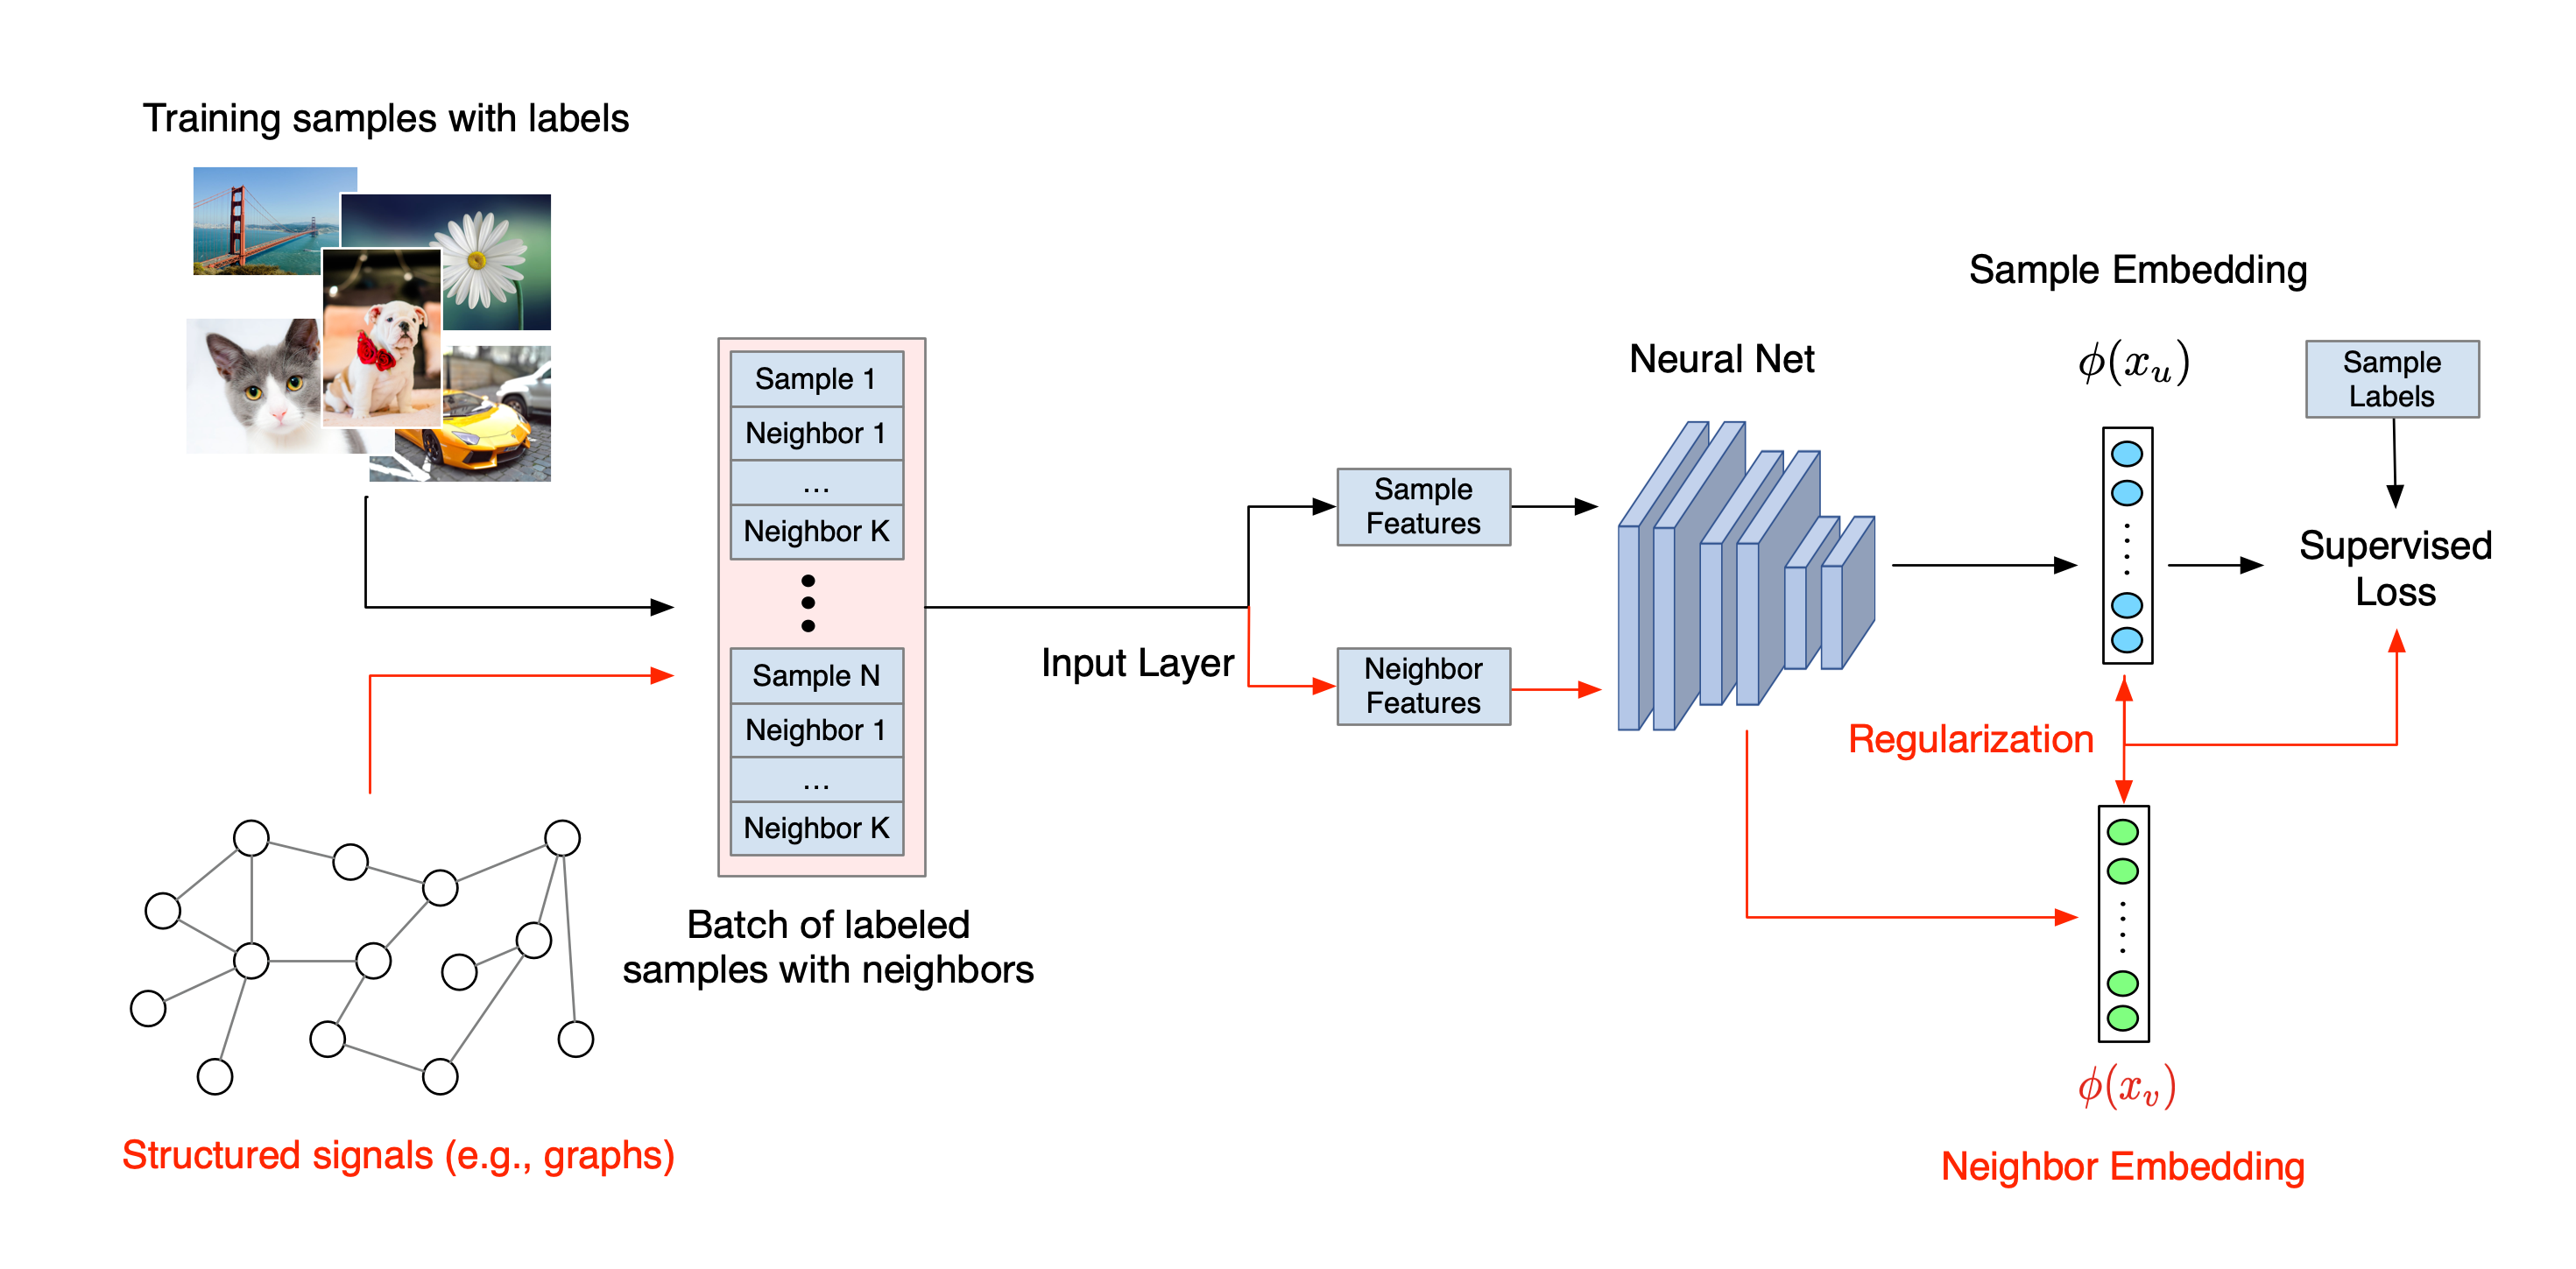
\includegraphics[width=0.8\linewidth]{Image/NSL.png}
    \caption {Neural Structured Learning}
    \label{Hình 1.2: Neural Structured Learning}
    \cite*{WEBSITE:4}
\end{figure}

Trong Neural Structured Learning (NSL), các tín hiệu có cấu trúc dù được xác định rõ ràng dưới dạng biểu đồ hay được học ngầm dưới dạng cách ví dụ đối nghịch được 
được sử dụng để thường xuyên đào tạo mạng neural, buộc mô hình phải học các dự đoán chính xác (bằng cách giảm thiểu mất mát có giám sát), đồng thời duy trì sự giống nhau giữa các đầu vào từ 
cùng một cấu trúc(bằng cách giảm thiểu tổn thất lân cận). Kỹ thuật này là chung và có thể được áp dụng trên các kiến trúc neural tùy ý, chẳng hạn như Feed-Forward NNs, CNNs, RNNs. 


\subsection{Neural Graph Learning}

\textbf{Training with natural graphs}

\begin{figure}[h!]
    \centering
    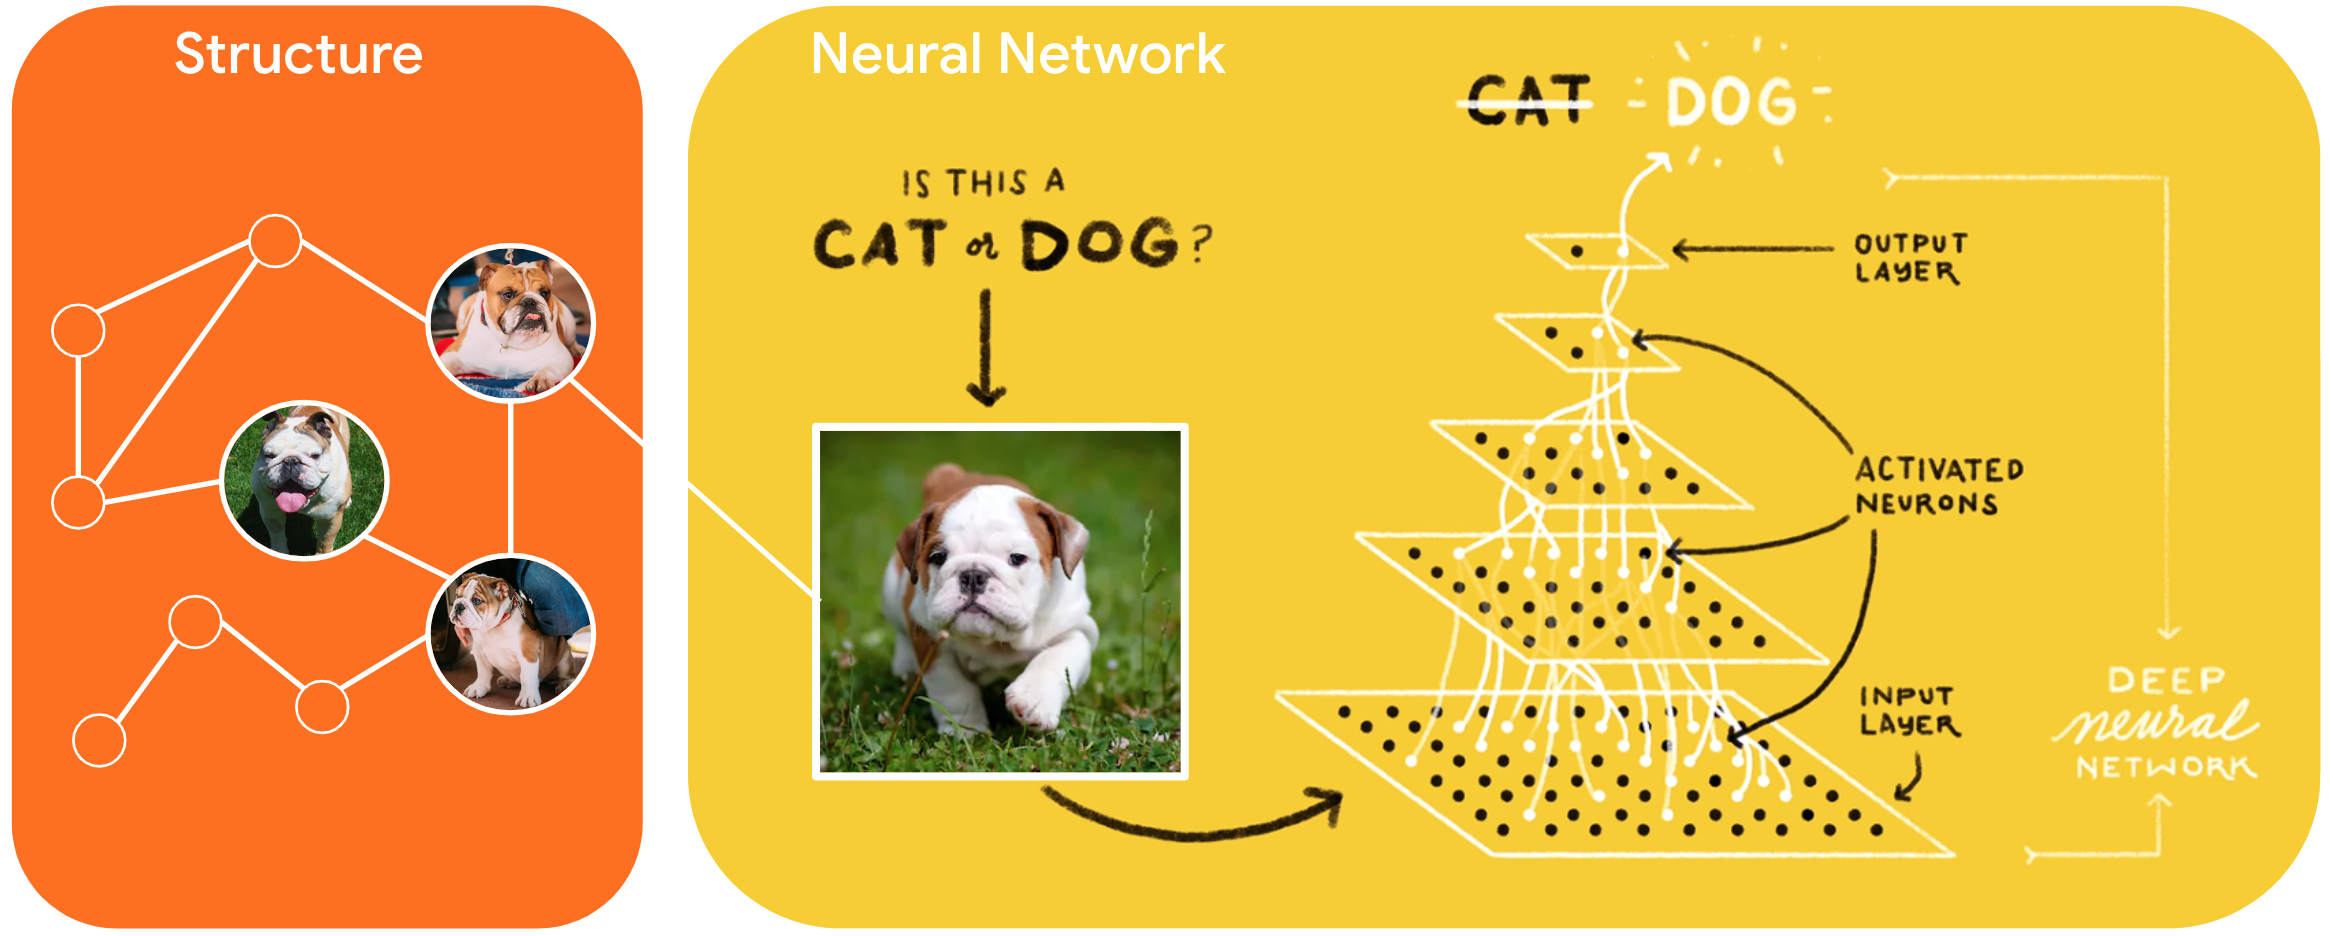
\includegraphics[width=0.8\linewidth]{Image/nsl_overview.png}
    \caption{Training with natural graphs}
    \label{Hình 1.3: Training with natural graphs}
    \cite*{WEBSITE:4}
\end{figure}

Về cơ bản, đồ thị tự nhiên là một tập hợp các điểm dữ liệu có mối quan hệ mật thiết với nhau, bản chất của mối quan hệ này có thể thay đổi dựa trên bối cảnh.
Mạng xã hội và Web là những ví dụ kinh điển mà chúng ta tương tác hàng ngày, ngoài những ví dụ này, chúng còn thường xuất hiện trong dữ liệu thường được sử dụng
cho nhiều nhiệm vụ học máy. Ví dụ khi ta cố gắng nắm bắt hành vi của người dùng dựa trên tương tác của họ với dữ liệu, thì việc lập mô hình dữ liệu dưới dạng biểu đồ 
có thể hợp lý. Đối với xử lý ngôn ngữ tự nhiên, chúng ta có thể định nghĩa một biểu đồ văn bản trong đó các nút biểu thị các thực thể và các cạnh biểu thị mối quan hệ 
giữa các cặp thực thể.

Xem xét bài toán phân loại tài liệu. Ví dụ như những kỹ sư AI thường chỉ quan tâm đến các bài viết về học máy trên một chủ đề cụ thể như thị giác máy tính hoặc xử lý ngôn ngữ
tự nhiên hoặc học tăng cường. Và thông thường, chúng ta có rất nhiều tài liệu hoặc giấy tờ như thế để phân loại, nhưng rất ít trong số chúng có nhãn. Vì vậy cần phải làm cho 
dữ liệu được thiết lập thành một biểu đồ tự nhiên, điều này nghĩa là nếu một bài báo hoặc tài liệu được trích dẫn từ bài báo hoặc tài liệu khác thì chúng có thể có cùng nhãn.
Việc sử dụng các thông tin quan hệ như vậy từ biểu đồ trích dẫn tận dụng được cả các mẫu được gắn nhãn cũng như không được gẵn nhãn. Điều này có thể bù đắp cho việc thiếu nhãn 
trong dữ liệu đào tạo. Vì vậy, việc xây dựng các đồ thị tự nhiên là rất cần thiết để giúp đào tạo các mô hình học máy một cách hiệu quả hơn.

\textbf{Traning with synthesized graphs}

\begin{figure}[h!]
    \centering
    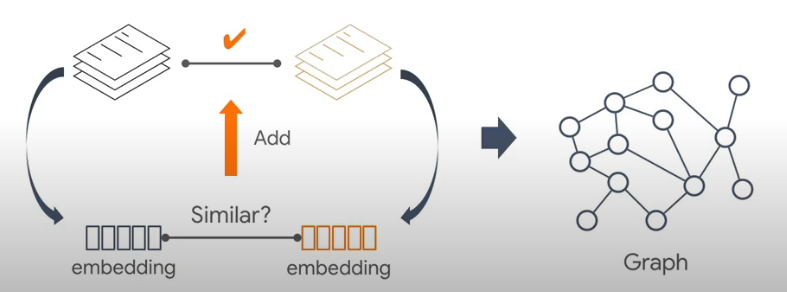
\includegraphics[width=0.8\linewidth]{Image/Graph2.png}
    \caption{Traning with synthesized graphs}
    \label{Hình 1.3: Traning with synthesized graphs}
    \cite*{WEBSITE:4}
\end{figure}

Mặc dù đồ thị tự nhiên là phổ biến, tuy nhiên có nhiều bài toán học máy với dữ liệu đầu vào không tạo thành đồ thị tự nhiên.
Ví dụ như phân loại văn bản đơn giản hoặc phân loại hình ảnh thì dữ liệu đầu vào chỉ chứa hình ảnh hoặc văn bản thô, do đó ta không thể 
tạo ra biểu đồ tự nhiên. Vì vậy Training with synthesized graphs được sử dụng để giải quyết vấn đề này. Với ý tưởng chính là xây dựng hoặc tổng hợp một biểu đồ từ dữ liệu đầu vào.
Trong Training with synthesized graphs chúng ta vẫn sự dụng sự giống nhau giữa các dữ liệu để xây dựng biểu đồ. Để xác định số liệu tương tự, thì cần phải chuyển đổi các văn bản thô hoặc
hình ảnh thành các thành phần nhúng tương ứng hoặc các biểu diễn dày đặc. Khi chuyển đổi dữ liệu thành các thành phần nhúng tương ứng, thì ta có thể sử dụng các mô hình đào tạo trước đó hoặc 
một số hàm chẳng hạn như cos để so sánh mức độ tương ứng giữa của các cặp phần nhúng. Nếu điểm tương đồng lớn hơn một ngưỡng nhất định thì ta sẽ thêm vào một cạnh tương ứng vào biểu đồ kết quả.
Việc lặp lại quy trình này sẽ bao phủ toàn bộ tập dữ liệu và sẽ tạo ra một biểu đồ. Và khi ta có biểu đồ thì việc sử dụng phương pháp học có cấu trúc trung tính rất đơn giản.


\subsection{Adversarial Learning}

\subsubsection*{Adversarial examples}

Adversarial example là các mẫu được tạo ra với những thao tác tinh vi bằng cách thêm vào các nhiễu đối nghịch nhỏ mà mắt người không thể nào nhìn thấy được đã biến nó thành một hình ảnh hoàn toàn khác dưới con mắt kỹ thuật số của thuật 
toán machine learning.

Một số mô hình học máy bao gồm các mạng lưới thần kinh hiện đại nhất, dễ bị sai lệch trước những Adversarial examples. Những mô hình này cho ra kết quả sai các ví dụ chỉ khác một chút so với các ví dụ được phân loại chính xác từ trong tập 
dữ liệu. Ví dụ như khi chúng ta đưa ra đặc điểm của một con gấu trúc thì chúng ta sẽ tìm những đặc trưng của nó như mắt đen, đầu tròn, thân trắng... Nhưng đối với một mạng neural nhân tạo, miễn là khi dữ liệu được đưa vào chạy qua các layer 
đưa ra kết quả trả lời đúng thì nó sẽ tin hình ảnh của dữ liệu đó là con gấu trúc.

\begin{figure}[h!]
    \centering
    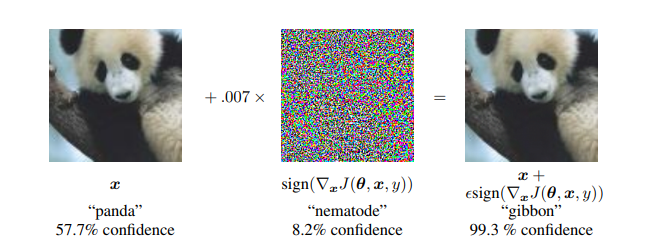
\includegraphics[width=0.8\linewidth]{Image/ADV.png}
    \caption{Adversarial examples}
    \label{Hình 1.4: Adversarial examples}
    \cite*{Reference7}
\end{figure}

Từ hình 2.4 ta thấy, khi thêm vào 1 vector tín hiệu nhiễu rất rất bé mà mắt người không thể phân biệt được sự khác nhau giữa hai hình ảnh của con gấu trúc thì nó đã đánh lừa được mạng neural và khiến nó phán đoán sai và nó tin chắc rằng
thứ mà nó đang nhìn thấy là con vượn (99.3\%). Điều này cho thấy khi các tập dữ liệu không tốt(có nhiễu) thì có thể khiến mạng neural đưa ra phán đoán sai.
 Để giải quyết vấn đề này, Adversarial training được đề xuất để dạy các mạng neural không bị đánh lừa và phân loại sai. 

\cite*{Reference6}
\textbf{Adversarial training}

Khái niệm về Adversarial training liên quan đến việc đào tạo bộ phân loại để khái quát hóa
Adversarial examples cũng như mẫu sạch. Trong lược đồ đào tạo thông thường, được hiển thị trong Hình 2.5, dữ liệu đào tạo chuyển tiếp
thông qua mô hình và tổn thất dự đoán được lan truyền ngược để cải thiện phân loại
kết quả. Kết quả là, mô hình sẽ khái quát hóa việc phân phối dữ liệu huấn luyện để
đưa ra một dự đoán chính xác về nhãn. 

Để đào tạo mô hình tránh bị nhầm lẫn khi tập dữ liệu có nhiễu thì ta sẽ tạo ra các dữ liệu có nhiễu nhỏ từ tập dữ liệu đào tạo
sau đó thêm các cạnh để kết nối dữ liệu vừa tạo ra với các mẫu của nó để xây dựng một cấu trúc linh hoạt sau đó, cấu trúc này có thể được sử dụng trong khung học tập
của cấu trúc thần kinh. Trong khung học cấu trúc thần kinh, mạng thần kinh cố gắng học cách duy trì cấu trúc bằng cách giữ sự giống nhau giữa một mẫu và hàng xóm của nó.
 Vì vậy về cơ bản việc sử dụng tập dữ liệu sạch và dữ liệu đối nghịch của nó sẽ nói với mạng thần kinh rằng mẫu và mẫu đối nghịch của nó thực sự giống nhau. Vì vậy, hãy giữ sự 
 giống nhau giữa chúng và đừng bị nhầm lẫn bởi các nhiễu.

\begin{figure}[h!]
    \centering
    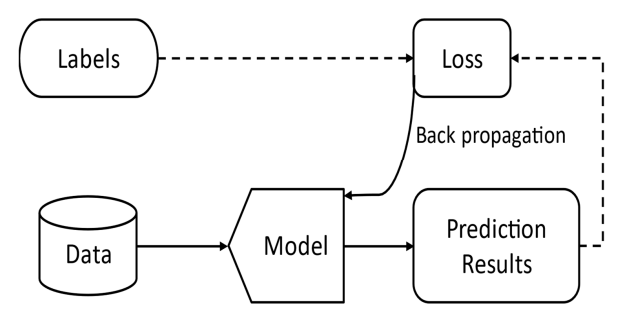
\includegraphics[width=0.72\linewidth]{Image/ADVT1.png}
    \caption{Basic training}
    \label{Hình 2.5: Adversarial training}
    \cite*{Reference8}
\end{figure}

Adversarial training mở rộng các phương pháp đào tạo thông thường bằng cách bổ sung thêm
bước vào quy trình đào tạo, như được minh họa trong Hình 2.6. Bằng cách này, mô hình có thể
khái quát hóa cả dữ liệu sạch và dữ liệu đối nghịch được tạo ra bởi các phương thức
được sử dụng trong Adversarial training để chống lại sự đánh lừa của mẫu đối nghịch.

\begin{figure}[h!]
    \centering
    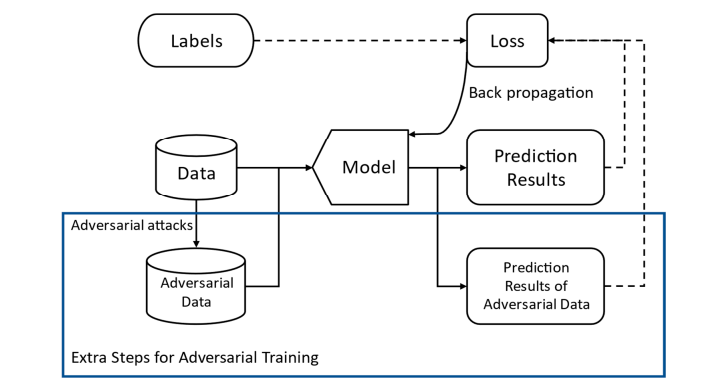
\includegraphics[width=0.72\linewidth]{Image/ADVT2.png}
    \caption{Adversarial training}
    \label{Hình 2.6: Adversarial training}
    \cite*{Reference8}
\end{figure}

Trong thư viện TensorFlow có sẵn các hàm chức năng để tạo ra các mẫu đối ngịch. 
Tương tự thì Keras API cũng có thể sử dụng để cho phép đào tạo từ đầu đến cuối
một cách dễ dàng với Adversarial training như: AdversarialRegularization, AdvNeighborConfig, AdvRegConfig...

\section{Adversarial Regularization for Image Classification}
\subsection{Chuẩn bị dữ liệu}

Ở phần trước chúng ta đã đi qua tổng quan về TensorFLow và Neural Structured Learning. Tuy nhiên để làm rõ hơn về hiệu quả của Neural
Structured Learning, chúng ta cần thực nghiệm trên một bài toán thực tế. Vì vậy ta sẽ ứng dụng Neural Structured Learning và chính xác hơn là Adversarial 
Regularization for Image Classification.
\begin{figure}[h!]
    \centering
    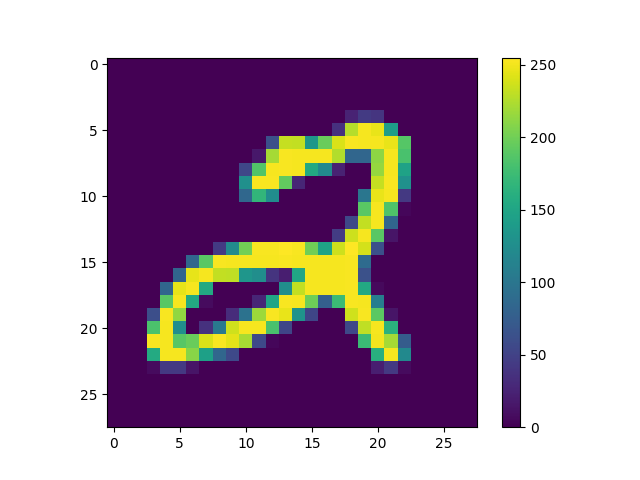
\includegraphics[width=0.6\linewidth]{Image/data.png}
    \caption{Ảnh chữ số viết tay được lấy từ tập dữ liệu MNIST}
    \label{Hình 2.7: GẢnh chữ số viết tay được lấy từ tập dữ liệu MNIST}
\end{figure}


Dựa trên tập dữ liệu có sẵn của thư viện TensorFlow MNIST, chúng ta sẽ thực hiện một bài toán phân loại ảnh chữ số viết tay. Tập dữ liệu bao gồm 70.000 ảnh
chữ số viết tay được chia thành 60.000 ảnh để huấn luyện và 10.000 ảnh để kiểm tra. Mỗi ảnh có kích thước 28x28 pixel và được biểu diễn dưới dạng một mảng
2 chiều 28x28. Mỗi phần tử trong mảng này là một giá trị từ 0 đến 255 biểu diễn độ sáng của một pixel. Để thuận tiện cho việc huấn luyện, chúng ta sẽ chuyển đổi
mỗi ảnh thành một mảng 1 chiều 784 phần tử. Để đơn giản hơn, chúng ta sẽ chia tập dữ liệu thành 2 tập huấn luyện và kiểm tra. Tập huấn luyện sẽ bao gồm 60.000 ảnh 
và tập kiểm tra sẽ bao gồm 10.000 ảnh. Mỗi ảnh sẽ được gán nhãn là một số từ 0 đến 9 tương ứng với chữ số viết tay. 

\subsection{Mô hình}
Chúng ta có thể sử dụng các mạng neural thông thường để xây dựng mô hình phán đoán chữ số. Ý tưởng là sử dụng một vài mạng neural để tính toán các trọng số
của mô hình. 
\begin{equation}
    \begin{aligned}  
      w_1X_1 + w_2X_2 + ... + w_nX_n = y\\
    \end{aligned}
\end{equation}

trong đó:
\begin{itemize}
    \item $w_1, w_2, ..., w_n$ là các trọng số của mô hình.
    \item $X_1, X_2, ..., X_n$ là giá trị của các pixel.
    \item $y$ là giá trị dự đoán của mô hình.
\end{itemize}


Mô hình sẽ tìm kiếm các trọng số phù hợp để đưa ra được đầu ra y chính xác đối với các hình ảnh đầu vào.
Tuy nhiên nếu thưc hiện như vậy, chúng ta sẽ không thể đạt được kết quả tốt. Vì vậy chúng ta cần phải sử dụng một số kỹ thuật để cải thiện độ chính xác của mô hình.
Bằng cách thêm các convolutional layer và pooling layer vào mô hình, chúng ta sẽ có thể giảm số lượng tham số của mô hình và cải thiện độ chính xác của mô hình.



Chúng ta sẽ thực hiện xây dựng và đào tạo một mạng neural đơn giản và một mạng neural sử dụng Adversarial Regularization. Sau đó chúng ta sẽ so sánh kết quả 
dự đoán của 2 mạng neural này để thấy được hiệu quả của Neural Structured Learning. Sau khi đào tạo và dự đoán thử trên tập dữ liệu có sẵn của TensorFlow, thì
ta sẽ thử viết tay một vài chữ số và để cho mạng neural dự đoán xem nó có thể dự đoán chính xác không.

Với những thư viện đồ sộ và khả năng làm việc với các ma trận tốt, Python là ngôn ngữ được lựa chọn để thực hiện ý tưởng trên. Cùng với đó là các thư viện như numpy, matplotlib và
đặc biệt là TensorFlow với API keras và Neural structed learning.



 
%% Template cho một chương

\chapter{Adversarial regularization for image classification} % Tên của chương

\label{Chapter2} % Thay X bằng số chương tương ứng; để trích dẫn chương này ở chỗ nào đó trong bài, hãy sử dụng lệnh \ref{ChapterX} 

%----------------------------------------------------------------------------------------
%	MỤC 1
%----------------------------------------------------------------------------------------

\section{Đặt vấn đề}

Ở chương một chúng ta đã đi qua tổng quan về TensorFLow và Neural Structured Learning. Tuy nhiên để làm rõ hơn về hiệu quả của Neural
Structured Learning, chúng ta cần thực nghiệm trên một bài toán thực tế. Vì vậy ta sẽ ứng dụng Neural Structured Learning và chính xác hơn là Adversarial 
Regularization for Image Classification.

Dựa trên tập dữ liệu có sẵn của thư viện TensorFlow MNIST, chúng ta sẽ thực hiện một bài toán phân loại ảnh chữ số viết tay. Tập dữ liệu bao gồm 70.000 ảnh
chữ số viết tay được chia thành 60.000 ảnh để huấn luyện và 10.000 ảnh để kiểm tra. Mỗi ảnh có kích thước 28x28 pixel và được biểu diễn dưới dạng một mảng
2 chiều 28x28. Mỗi phần tử trong mảng này là một giá trị từ 0 đến 255 biểu diễn độ sáng của một pixel. Để thuận tiện cho việc huấn luyện, chúng ta sẽ chuyển đổi
mỗi ảnh thành một mảng 1 chiều 784 phần tử. Để đơn giản hơn, chúng ta sẽ chia tập dữ liệu thành 2 tập huấn luyện và kiểm tra. Tập huấn luyện sẽ bao gồm 60.000 ảnh 
và tập kiểm tra sẽ bao gồm 10.000 ảnh. Mỗi ảnh sẽ được gán nhãn là một số từ 0 đến 9 tương ứng với chữ số viết tay. 

\begin{figure}[h!]
    \centering
    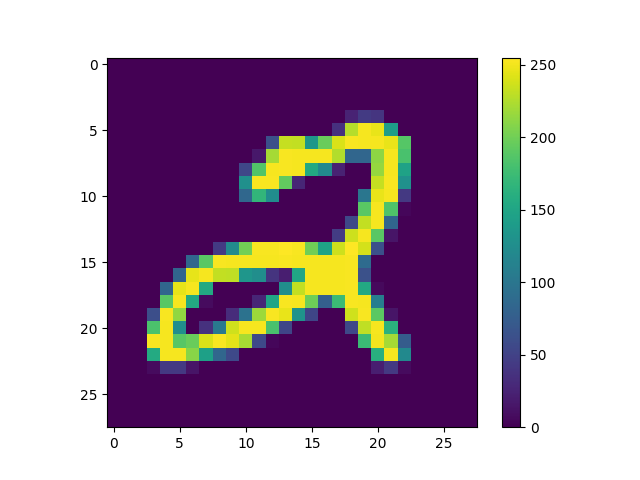
\includegraphics[width=0.6\linewidth]{Image/data.png}
    \caption{Ảnh chữ số viết tay được lấy từ tập dữ liệu MNIST}
    \label{Hình 2.1: GẢnh chữ số viết tay được lấy từ tập dữ liệu MNIST}
\end{figure}


Chúng ta sẽ thực hiện xây dựng và đào tạo một mạng neural đơn giản và một mạng neural sử dụng Adversarial Regularization. Sau đó chúng ta sẽ so sánh kết quả 
dự đoán của 2 mạng neural này để thấy được hiệu quả của Neural Structured Learning. Sau khi đào tạo và dự đoán thử trên tập dữ liệu có sẵn của TensorFlow, thì
ta sẽ thử viết tay một vài chữ số và để cho mạng neural dự đoán xem nó có thể dự đoán chính xác không.

Với những thư viện đồ sộ và khả năng làm việc với các ma trận tốt, Python là ngôn ngữ được lựa chọn để thực hiện ý tưởng trên. Cùng với đó là các thư viện như numpy, matplotlib và
đặc biệt là TensorFlow với API keras và Neural structed learning.





%----------------------------------------------------------------------------------------
%	MỤC 2
%----------------------------------------------------------------------------------------

\section{Thực nghiệm}

\subsection{Cài đặt môi trường}

Bước đầu tiên cần cài đặt biến môi trường và các thư viện cần thiết. Cài đặt phiên bản python3 và editor hoặc IDE để viết mã như Pycharm hoặc VScode.
Sau đó, trên command line chạy dòng lệnh 'pip install -r Setup.txt' để tiến hành cài đặt các thư viện cần thiết. File "Setup.txt" là file chứa các thư viện 
cần cài đặt.

\subsection{Viết mã}
\textbf{Import thư viện}
% insert code python
\begin{lstlisting}[language=Python]
    import tensorflow as tf
    import numpy as np
    import neural_structured_learning as nsl
    import matplotlib.pyplot as plt
    import tensorflow_datasets as tfds
\end{lstlisting}

\textbf{Khai báo các tham số}
% insert code python
\begin{lstlisting}[language=Python]
    input_shape = [28, 28, 1]
    num_classes = 10
    conv_filters = [32, 64, 64]
    kernel_size = (3, 3)
    pool_size = (2, 2)
    num_fc_units = [64]
    batch_size = 32
    epochs = 5
    adv_multiplier = 0.2
    adv_step_size = 0.2
    adv_grad_norm = 'infinity'
\end{lstlisting}

Khai báo các tham số cần thiết cho việc xây dựng mạng neural và đào tạo. Các tham số được khai báo như sau:

Đầu vào và đầu ra:
\begin{itemize}
    %highlight Item name
    \item \textbf{input\_shape}: Hình dạng của tensor đầu vào. Mỗi hình ảnh có kích thước 28x28pixel và có 1 kênh màu.
    \item \textbf{num\_classes}: Số lượng lớp đầu ra. Trong bài toán này là 10 lớp từ 0 đến 9.
\end{itemize}

Các tham số để xây dựng mô hình mạng neural:
\begin{itemize}
    %highlight Item name
    \item \textbf{conv\_filters}: Số lượng lọc cho mỗi lớp tích chập. Mỗi lớp tích chập có số bộ lọc bao gồm 32,64,64.
    \item \textbf{kernel\_size}: Kích thước của kernel tích chập 2D. Mỗi kernel có kích thước 3x3.
    \item \textbf{pool\_size}: Các yếu tố để thu nhỏ hình ảnh trong mỗi lớp tổng tối đa. Mỗi pooling có kích thước 2x2.
    \item \textbf{num\_fc\_units}: Số lượng đơn vị ẩn của mỗi lớp fully connected. Mỗi lớp fully connected có 64 đơn vị ẩn. Nghĩa là chiều rộng của mỗi lớp được kết nối đầy đủ.
\end{itemize}

Các tham số để đào tạo mô hình:
\begin{itemize}
    \item \textbf{batch\_size}: Kích thước batch. Mỗi batch có 32 hình ảnh. Là số lượng bức ảnh được đưa vào mạng neural mỗi lần.
    \item \textbf{epochs}: Số lần huấn luyện. Mỗi lần sẽ duyệt qua tất cả các hình ảnh trong tập dữ liệu.
    \item \textbf{adv\_multiplier}: Trọng số tổn thất do nhiễu loạn đối nghịch gây ra trong mục tiêu huấn luyện, so với tổn thất của mô hình gốc(tổn thất được gắn nhãn).
    \item \textbf{adv\_step\_size}: Độ lớn của nhiễu loạn đối nghịch.
    \item \textbf{adv\_grad\_norm}: Định mức để đo mức độ nhiễu loạn của đối nghịch. %Có 3 giá trị là 'infinity', 'l2', 'l1'.
\end{itemize}

\textbf{Tải dữ liệu MNIST}
% insert code python
\begin{lstlisting}[language=Python]
    data_train, data_test = tfds.load('mnist', split=['train', 'test'])
\end{lstlisting}

Bộ dữ liệu MNIST chứa hình ảnh thang độ xám của các chữ số viết tay từ 0 dến 9. Mỗi hình ảnh hình ảnh hiển thị một chữ số ở độ phân giải thấp 28x28 pixel.
Nhiệm vụ liên quan là phân loại hình ảnh thành 10 loại, mỗi loại tương ứng với một chữ số từ 0 đến 9.

Bộ dữ liệu đã có sẵn trong thư viện TensorFlow Datasets (TFDS) và có thể được tải xuống và xây dựng tệp tf.data.Dataset.
Tập dữ liệu đã tải bao gồm hai tập con :
\begin{itemize}
    \item \textbf{train}: Tập dữ liệu huấn luyện với 60000 ảnh.
    \item \textbf{test}: Tập dữ liệu kiểm tra với 10000 ảnh.
\end{itemize}

Các dữ liệu trong cả hai tập đều được lưu trữ dưới dạng dictionary với hai khóa:
\begin{itemize}
    \item \textbf{image}: Là các mảng pixel 28x28 chứa các giá trị từ 0 đến 255.
    \item \textbf{label}: Nhãn thật của hình ảnh, là một số nguyên từ 0 đến 9.
\end{itemize}

\begin{lstlisting}[language=Python]
    def normalize(features):
        features['image'] = tf.cast(features['image'], dtype=tf.float32) / 255.0
        return features

    def convert_to_tuples(features):
        return features['image'], features['label']

    def convert_to_dictionaries(image, label):
        return {'image': image, 'label': label}

    data_train = data_train.map(normalize).shuffle(10000).batch(batch_size).map(convert_to_tuples)
    data_test = data_test.map(normalize).batch(batch_size).map(convert_to_tuples)

\end{lstlisting}

Để làm cho mô hình ổn định về số lượng, chúng ta chuẩn hóa các giá trị pixel từ [0,255] thành [0, 1] bằng cách ánh xạ tập dữ liệu qua hàm normalize(). Sau khi xáo 
trộn tập huấn luyện và chia theo nhóm, chúng ta chuyển đổi các ví dụ thành các bộ dữ liệu đặc trưng (image, label) để huấn luyện mô hình cơ sở. Chúng ta 
cũng cung cấp một hàm chức năng để chuyển đổi từ bộ sang từ điển để sử dụng sau này.

\textbf{Xây dựng và đào tạo mô hình cơ bản}

Mô hình cơ bản sẽ là một mạng thần kinh bao gồm 3 lớp tích chập, theo sau là 2 lớp được kết nối đầy đủ ( với các tham số như được định nghĩa trong phần khai báo tham số). 
Trong đó các lớp tích chập sẽ có hàm kích hoạt activation là 'relu' còn hai lớp theo sau thì một lớp có hàm kích hoạt là 'relu'và lớp output sẽ là 'softmax'. Lớp output sử dụng 
activation 'softmax' để đánh giá xác suất phân loại dữ liệu đầu vào và tính toán trọng số cho dữ liệu.
Chúng ta tạo hàm build\_model() để thuận tiện cho việc tái sử dụng khi khởi tạo mô hình khác. 
Ở đây chúng ta xác định nó bằng các hàm API của Keras. 

\begin{lstlisting}[language=Python]
    def build_model():
        inputs = tf.keras.Input(shape=input_shape, dtype=tf.float32, name='image')
        x = inputs
        for i, num_filters in enumerate(conv_filters):
            x = tf.keras.layers.Conv2D(num_filters, kernel_size, activation='relu')(x)
            if i < len(conv_filters) - 1:
                x = tf.keras.layers.MaxPooling2D(pool_size)(x)
        x = tf.keras.layers.Flatten()(x)
        for num_units in num_fc_units:
            x = tf.keras.layers.Dense(num_units, activation='relu')(x)
        outputs = tf.keras.layers.Dense(num_classes, activation='softmax')(x)
        return tf.keras.Model(inputs=inputs, outputs=outputs)

    model_base = build_model()
\end{lstlisting}

Sau khi xây dựng model thì chúng ta sẽ tiến hành đào tạo và đánh giá model. Với hàm tối ưu hóa 'Adam' như đã giới thiệu ở phần trước, hàm mất mát 'SparseCategoricalCrossentropy'
và đánh giá 'SparseCategoricalAccuracy'. Sau khi đào tạo xong chúng ta sẽ đánh giá model bằng hàm evaluate() và in ra độ chính xác của model.

\begin{lstlisting}[language=Python]
model_base.compile(
    optimizer=tf.keras.optimizers.Adam(),
    loss=tf.keras.losses.SparseCategoricalCrossentropy(),
    metrics=[tf.keras.metrics.SparseCategoricalAccuracy()])
model_base.summary()

model_base_history = model_base.fit(data_train, epochs=epochs)

results = model_base.evaluate(data_test)
named_results = dict(zip(model_base.metrics_names, results))
print('\naccuracy:', named_results['sparse_categorical_accuracy'])

\end{lstlisting}

\begin{figure}[ht]
\centering
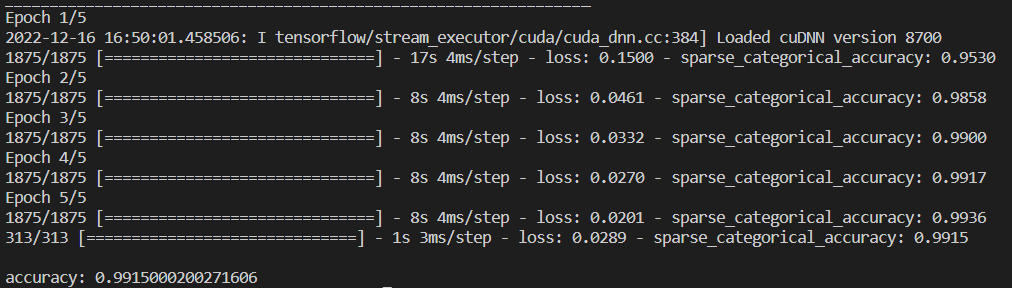
\includegraphics[width=\textwidth]{Image/base_acc.png}
\caption{Accuracy}
\label{fig2.2:Độ chính xác của mô hình cơ bản}
\end{figure}

Chúng ta có thể thấy rằng mô hình cơ bản đạt được độ chính xác lên đến 99,15\% trên bộ thử nghiệm. Từ đó cho thấy dữ liệu đào tạo và 
mô hình đào tạo là khá tốt. Tuy nhiên cần phải sử dụng các tập dữ liệu khác để đánh giá mô hình một cách chính xác hơn.

\textbf{Xây dựng và đào tạo mô hình Adversarial-regularized }

Chúng ta sẽ xây dựng mô hình mạng neural đối nghịch bằng cách kết hợp adversarial training vào mô hình keras và sử dụng khung Neural Structured Learning (NSL).
Mô hình cơ sở được bao bọc để tạo một mô hình mới \textbf{tf.Keras.Model}, có mục tiêu đào tạo bao gồm adversarial regularization.

Đầu tiên, chúng tôi tạo một đối tượng cấu hình với tất cả cáctham số có liên quan bằng cách sử dụng hàm chức năng \textbf{nsl.configs.make\_adv\_reg\_config} có sẵn trong thư viện NSL.

\begin{lstlisting}[language=Python]
    adv_config = nsl.configs.make_adv_reg_config(multiplier=adv_multiplier, 
        adv_step_size=adv_step_size, 
        adv_grad_norm=adv_grad_norm)
\end{lstlisting}

Ở đây chúng ta sẽ tạo một mô hình cơ bản mới \textbf{base\_adv\_model} để mô hình hiện tại (\textbf{model\_base}) dùng để so sánh sau này.

Bây giờ chúng ta có thể bọc một mô hình cơ sở bằng \textbf{AdversarialRegularization} bằng cách sử dụng hàm chức năng
có sẵn \textbf{nsl.keras.AdversarialRegularization}.

\begin{lstlisting}[language=Python]
    base_adv_model = build_model()
    model_adv = nsl.keras.AdversarialRegularization(
        base_adv_model,
        label_keys=['label'],
        adv_config=adv_config)

    data_train_adv = data_train.map(convert_to_dictionaries)
    data_test_adv = data_test.map(convert_to_dictionaries)
\end{lstlisting}

Trả về \textbf{adv\_model} là một đối tượng có kiểu \textbf{tf.keras.Model}, có mục tiêu đào tạo bao gồm phần regularization và mất mát của adveresarial. Để tính toán tổn thất đó, mô hình phải có quyền truy cập 
vào thông tin nhãn (feature label), ngoài đầu vào thông thường (feature image). Vì lý do này, chúng ta sẽ chuyển đổi các mẫu trong tập dữ liệu trở lại kiểu dictionary. Và chúng ta cho mô 
hình biết tính năng nào chứa thông tin nhãn thông qua tham số \textbf{label\_keys}.

Tiếp theo, chúng ta sẽ biên dịch, đào tạo và đánh giá mô hình chính quy hóa đối thủ. Với các hàm tối ưu, mất mát, và đánh giá độ chính xác tương tự như khi đào tạo mô hình cơ bản.
Có thể có các cảnh báo như "Output missing from loss dictionary", điều này không sao cả vì \textbf{adv\_model} không dựa vào triển khai cơ sở để tính tổng tổn thất.



\begin{lstlisting}[language=Python]
    model_adv.compile(
        optimizer=tf.keras.optimizers.Adam(),
        loss=tf.keras.losses.SparseCategoricalCrossentropy(),
        metrics=[tf.keras.metrics.SparseCategoricalAccuracy()])

    model_adv_history = model_adv.fit(data_train_adv, epochs=epochs)
    
    adv_results = model_adv.evaluate(data_test_adv)
    named_adv_results = dict(zip(model_adv.metrics_names, adv_results))
    print('\naccuracy:', named_adv_results['sparse_categorical_accuracy'])

\end{lstlisting}

\begin{figure}[h!]
    \centering
    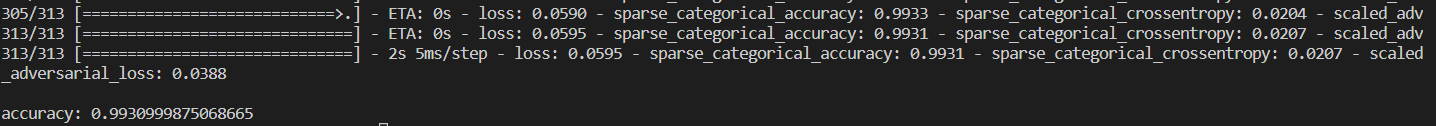
\includegraphics[width=\textwidth]{Image/adv_acc.png}
    \caption{Độ chính xác của mô hình Adversarial-regularized.}
    \label{fig 2.3:Độ chính xác của mô hình Adversarial-regularized}
\end{figure}

Chúng ta có thể thấy rằng mô hình Adversarial-regularized cũng hoạt động rất tốt (độ chính xác 99,31\%) trên tập thử nghiệm. Tuy độ chính xác có nhỉnh hơn một xíu so với mô hình cơ bản
nhưng không quá nhiều.

Chúng ta sẽ đưa ra đồ thị sự thay đổi của độ chính xác qua mỗi lần học tập trên tập dữ liệu thử nghiệm của cả hai mô hình để dễ dàng quan sát hơn.
\begin{lstlisting}[language=Python]
    plt.plot(model_base_history.history['sparse_categorical_accuracy'])
    plt.plot(model_adv_history.history['sparse_categorical_accuracy'])
    plt.title('model accuracy')
    plt.ylabel('accuracy')
    plt.xlabel('epoch')
    plt.legend(['base', 'adversarial'], loc='upper left')
    plt.show()
\end{lstlisting}

\begin{figure}[h!]
    \centering
    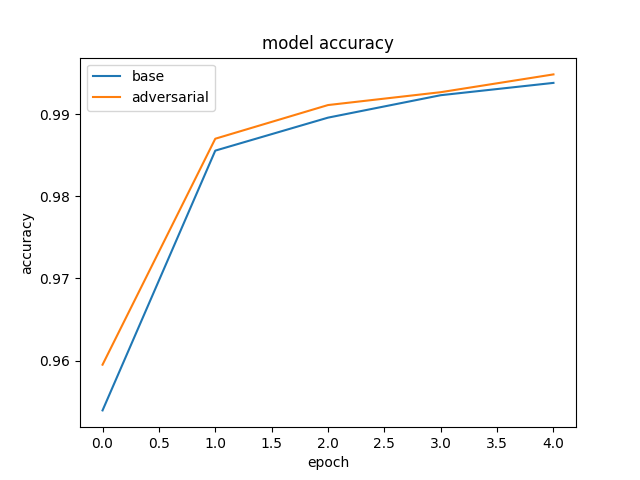
\includegraphics[width=0.7\textwidth]{Image/plt.png}
    \caption{Đồ thị độ chính xác của hai mô hình qua từng lần học.}
    \label{fig 2.4:Đồ thị độ chính xác của hai mô hình qua từng lần học.}
    
\end{figure}

Từ đồ thị, ta thấy đường cong độ chính xác của mô hình Adversarial-regularized và mô hình cơ bản có xu hướng tương tự nhau. Mô hình adversarial-regularized có nhỉnh hơn một chút nhưng chênh lệch là không quá nhiều. 
Điều này là do cả hai mô hình đều sử dụng các hàm tối ưu, mất mát và đánh giá tương tự nhau.

\textbf{So sánh độ chính xác của hai mô hình dưới các mẫu nhiễu loạn đối nghịch}

Bây giờ chúng ta so sánh mô hình cơ sở và mô hình Adversarial-regularized về khả năng phán đoán chính xác dưới sự nhiễu loạn của các mẫu đối nghịch.
Chúng ta sẽ sử dụng hàm chức năng \textbf{AdversarialRegularization.perturb\_on\_batch()} để tạo các mẫu nhiễu loạn đối nghịch. Để có thể sánh được độ chính xác của hai mô hình,
ta sẽ phải bọc mô hình cơ bản bằng \textbf{AdversarialRegularization}. Các biến mà mô hình cơ bản đã học trước đó sẽ không bị thay đổi miễn là chúng ta không gọi hàm đào tạo \textbf{fit()}.

\begin{lstlisting}[language = Python]
    ref_model = nsl.keras.AdversarialRegularization(
        model_base,
        label_keys=['label'],
        adv_config=adv_config)


    ref_model.compile(
        optimizer=tf.keras.optimizers.Adam(),
        loss=tf.keras.losses.SparseCategoricalCrossentropy(),
        metrics=[tf.keras.metrics.SparseCategoricalAccuracy()])
\end{lstlisting}

Tiếp theo chúng ta sẽ đánh giá và so sánh khả năng phán đoán của hai mô hình trên các mẫu đối nghịch.
Ở đây chúng ta lấy \textbf{adv\_model.base\_model} để có cùng định dạng đầu vào (không yêu cầu thông tin nhãn) làm mô hình cơ sở. Các biến đã học trong \textbf{adv\_model.base\_model} giống như các biến 
trong \textbf{adv\_model}.

\begin{lstlisting}[language = Python]
    models_to_evaluate = {
        'base': model_base,
        'adversarial': model_adv.base_model,
    }

    metrics = {
        name: tf.keras.metrics.SparseCategoricalAccuracy()
        for name in models_to_evaluate.keys()
    }    
\end{lstlisting}

Tiếp theo chúng ta sẽ tạo các ví dụ nhiễu loạn và đánh giá các mô hình với chúng. Chúng ta lưu các hình ảnh, nhãn và dự đoán bị nhiễu vào 3 mảng perturbed\_imgs,labels,predictions để trực 
quan hóa trong phần sau để có cách nhìn rõ hơn về khả năng phán đoán của hai mô hình. Các mẫu nhiễu loạn được tạo ra từ tập dữ liệu test và
được chuẩn hóa để chúng có cung kích thước với các mẫu thông thường bằng hàm chức năng \textbf{tf.clip\_by\_value}.


\begin{lstlisting}[language = Python]
    perturbed_imgs,labels,predictions = [],[],[]

    for batch in data_test_adv:
        perturbed_batch = ref_model.perturb_on_batch(batch)
        perturbed_batch['image'] = tf.clip_by_value(perturbed_batch['image'], 0, 1)

        y_true = perturbed_batch.pop('label')
        perturbed_imgs.append(perturbed_batch['image'].numpy())
        labels.append(y_true.numpy())
        predictions.append({})

        for name, model in models_to_evaluate.items():
            y_pred = model(perturbed_batch)
            metrics[name].update_state(y_true, y_pred)
            predictions[-1][name] = tf.argmax(y_pred, axis=-1).numpy()

    for name, metric in metrics.items():
        print(f'{name} accuracy: {metric.result().numpy()}')

\end{lstlisting}

\begin{figure}[h!]
    \centering
    
\includegraphics[width=\textwidth]{Image/acc.png}
    \caption{Độ chính xác của hai mô hình trên mẫu nhiễu loạn đối nghịch.}
    \label{fig 2.5:Độ chính xác của hai mô hình trên mẫu nhiễu loạn đối nghịch.}
    
\end{figure}

Từ hình 2.5 Chúng ta có thể thấy rằng độ chính xác của mô hình cơ bản giảm đáng kể (từ 99,15\% xuống còn khoảng 57,7\%) khi đầu vào bị nhiễu. Mặt khác, 
độ chính xác của mô hình Adversarial-regularized chỉ giảm một chút (từ 99,31\% xuống 96,2\%). Điều này chứng tỏ tính hiệu quả của việc học đối thủ trong 
việc cải thiện độ chính của mô hình và khả năng hoạt động tốt của mô hình trên những tập dữ liệu nhiều nhiễu.

\textbf{Trực quan hóa các mẫu nhiễu loạn đối nghịch}

Chúng ta sẽ chọn ra một batch ngẫu nhiên trong mảng perturbed\_imgs đã lưu ở trên để trực quan hóa, ở đây batch được chọn là batch thứ 5.
Sử dụng thư viện \textbf{matplotlib} để hiển thị các hình ảnh và hiển thị các dự đoán của hai mô hình và kiểm tra xem mô hình đoán có đúng không so với
nhãn thật.


\begin{lstlisting}[language = Python]
    batch_index = 5

    batch_images = perturbed_imgs[batch_index]
    batch_labels = labels[batch_index]
    batch_predictions = predictions[batch_index]

    n_columns = 5
    n_rows = (batch_size + n_columns - 1) // n_columns

    print('acc in batch %d: ' % batch_index, end='')
    for name,pred in batch_predictions.items():
        print('%s model: %d / %d' % (name, np.sum(batch_labels == pred), batch_size))

    plt.figure(figsize=(n_columns * 2, n_rows * 2))
    for i,(img,y) in enumerate(zip(batch_images, batch_labels)):
        y_base = batch_predictions['base'][i]
        y_adv = batch_predictions['adversarial'][i]
        plt.subplot(n_rows, n_columns, i + 1)
        plt.title('true: %d, base: %d, adv: %d' % (y, y_base, y_adv))
        plt.imshow(img)
        plt.axis('off')

    plt.tight_layout()
    plt.show()

    
\end{lstlisting}

\begin{figure}[h!]
    \centering
    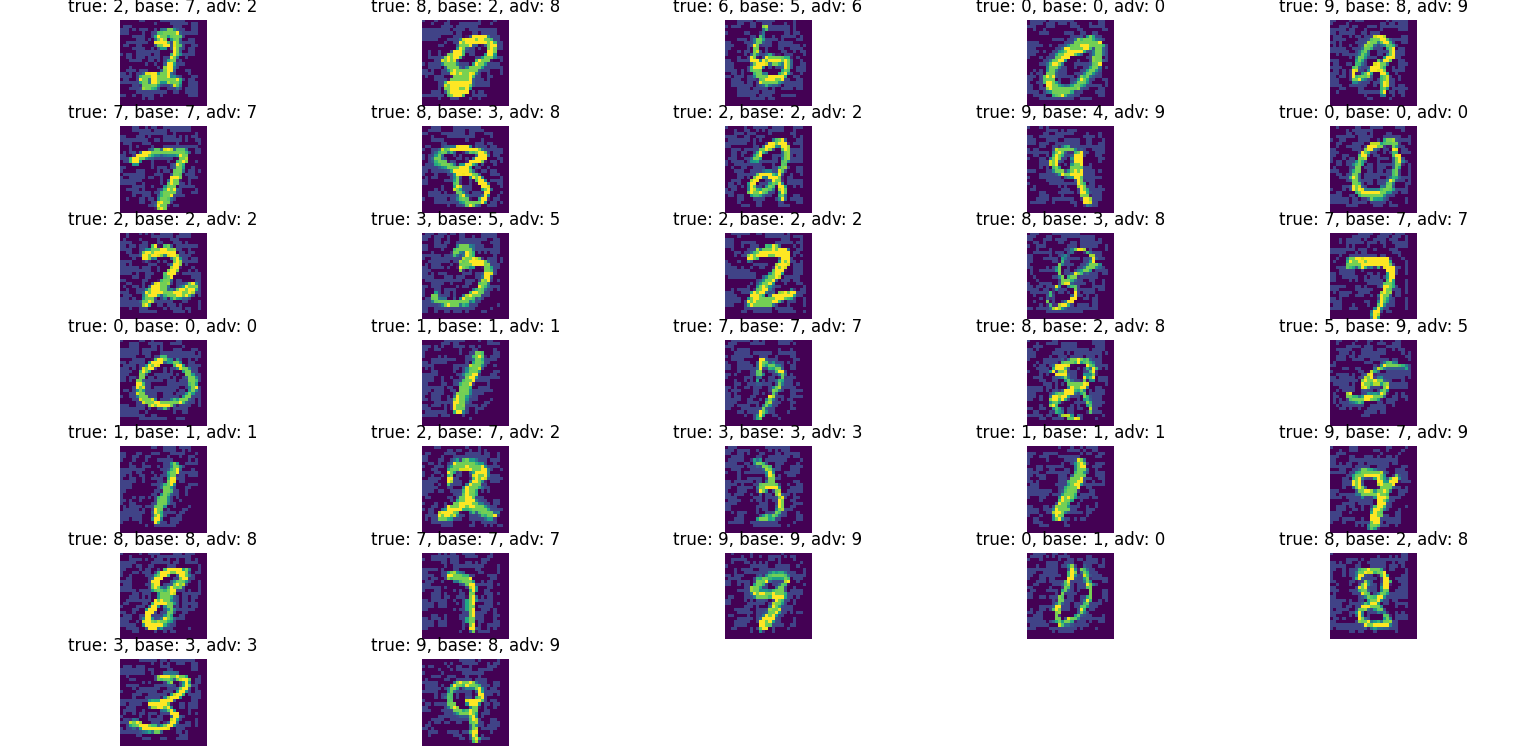
\includegraphics[width=\textwidth]{Image/result.png}
    \caption{Một số mẫu nhiễu loạn đối nghịch và các phán đoán của hai mô hình.}
    \label{fig 2.6:Một số mẫu nhiễu loạn đối nghịch và các phán đoán của hai mô hình.}
    
\end{figure}

\begin{figure}[h!]
    \centering
    
\includegraphics[width=\textwidth]{Image/acc_in_batch.png}
    \caption{Số dự đoán chính xác của hai mô hình trên mẫu nhiễu loạn đối nghịch trong batch 5.}
    \label{fig 2.7:Số dự đoán chính xác của hai mô hình trên mẫu nhiễu loạn đối nghịch trong batch 5.}
    
\end{figure}

Từ hình 2.6 ta thấy, các nhiễu loạn nhỏ được thêm vào những bức ảnh chữ số viết tay dưới mắt người vẫn có thể nhận biết được
tuy nhiên nó đã đánh lừa được mô hình cơ bản phán đoán sai.

Từ hình 2.7 ta thấy rằng, khả năng phán đoán của mô hình cơ bản(base model) khá thấp(21/32 mẫu). Trong khi đó
mô hình Adversarial-regularized phán đoán rất tốt (32/32 mẫu).


\textbf{Lưu mô hình vừa đào tạo}

Sau khi đào tạo chúng ta sẽ lưu lại các mô hình để thử cho các mô hình phán đoán một số hình ảnh viết tay không phải thuộc tập dữ
liệu của tensorflow\_datasets. Mô hình được lưu lại có thể dễ dàng mang ra sử dụng hoặc tiếp tục đào tạo tùy mục đích và no được lưu dưới định dạng '.h5' với sự hỗ trợ của
thư viện \textbf{h5py}. Lưu ý rằng, sau khi lưu mô hình thì các biến mà mô hình đã học tập được sẽ được giữ nguyên.

\begin{lstlisting}[language = Python]
    model_adv.save('Model/advs_model.h5')
    model_base.save('Model/base_model.h5')
\end{lstlisting}

\cite*{WEBSITE}

\subsection{Kiểm tra mô hình với một số ảnh viết tay}

Ở phần trước, chúng ta đã xây dựng, đào tạo và kiểm tra mô hình trên tập dữ liệu của tensorflow\_datasets. Tuy nhiên, chúng ta 
để biết được thực sự mô hình có hoạt động tốt với các bức ảnh ngẫu nhiên hay không, ta sẽ viết tay một số chữ số và cho mô hình dự đoán.

Ở phần này, chúng ta sẽ sử dụng thư viện xử lý ảnh OpenCV để đọc và tiền xử lý các bức ảnh chụp. Do đầu vào của mô hình là một bức ảnh 28x28
nên chúng ta cần phải resize ảnh về kích thước này. Sau đó, chúng ta cũng cần chuyển ảnh về dạng mảng numpy với giá trị trong khoảng 0-1 để mô hình ổn định hơn và 
tiến hành cho mô hình dự đoán.

\textbf{Import thư viện}

Các thư viện này đã được yêu cầu cài đặt trong file Setup.txt nên chỉ cần import vào là có thể sử dụng.
\begin{lstlisting}[language = Python]
    import cv2
    import numpy as np
    import tensorflow as tf
\end{lstlisting}

\textbf{Đọc ảnh và tiền xử lý ảnh}

Các bức ảnh chụp chữ số viết tay sẽ được lưu lại trong thư mục Image/. Chúng ta sẽ đọc các bức ảnh này và tiền xử lý để cho mô hình dự đoán.

\begin{lstlisting}[language = Python]
    image = cv2.imread("Image/test2.jpg")
    copy = image.copy()

    im_gray = cv2.cvtColor(image,cv2.COLOR_BGR2GRAY)
    im_blur = cv2.GaussianBlur(im_gray,(5,5),0)
    im,thre = cv2.threshold(im_blur,90,255,cv2.THRESH_BINARY_INV)
    contours,hierachy = cv2.findContours(thre,cv2.RETR_EXTERNAL,cv2.CHAIN_APPROX_SIMPLE)
    rects = [cv2.boundingRect(cnt) for cnt in contours]

\end{lstlisting}

Chúng ta sẽ đọc các bức ảnh này bằng hàm \textbf{imread()} có sẵn trong opencv sau đó sẽ copy ảnh vừa đọc và gán vào biến copy để sử dụng cho sau này.
Tiếp theo ta cần chuyển ảnh về dưới dạng thang xám để dễ dàng xử lý hơn bằng hàm \textbf{cvtColor()}.
Sau đó, chúng ta sẽ làm mờ ảnh bằng hàm \textbf{GaussianBlur()} để loại bỏ các nhiễu trong ảnh và tăng khả năng phán đoán chính xác của các mô hình.
Cuối cùng ta sẽ chuyển ảnh về dưới dạng nhị phân để có thể đưa vào mô hình dự đoán.

Do ảnh chụp có thể có nhiều chữ số viết tay nên chúng ta cần phải tách các chữ số ra. Để làm được điều này, chúng ta sẽ sử dụng hàm \textbf{findContours()} 
để tìm vị trí chuỗi số và các đường viền của các chữ số trong ảnh. Sau đó, chúng ta sẽ sử dụng hàm \textbf{boundingRect()} để tao các hình chữ nhật bao quanh các chữ số trong ảnh.

\textbf{Gọi mô hình và dự đoán}

Sau khi đã chuẩn bị các dữ liệu ảnh cần thiết, chúng ta sẽ gọi mô hình đã được train trước đó và dự đoán kết quả.

\begin{lstlisting}[language = Python]
    adv_model = tf.keras.models.load_model("Model/advs_model.h5")
    base_model = tf.keras.models.load_model("Model/base_model.h5")

    for i in contours:
        (x,y,w,h) = cv2.boundingRect(i)
        cv2.rectangle(image,(x,y),(x+w,y+h),(0,255,0),3)
        subImage = thre[y:y+h,x:x+w]
        subImage = np.pad(subImage,(20,20),'constant',constant_values=(0,0))
        subImage = cv2.resize(subImage, (28, 28), interpolation=cv2.INTER_AREA)
        subImage = cv2.dilate(subImage, (3, 3))

        img = subImage.reshape(1,28,28,1)
        img = img/255.0
        img = img.astype(np.float32)
        
        adv_pred = adv_model.predict(img)
        adv_pred = np.argmax(adv_pred)
        cv2.putText(copy,str(int(adv_pred)),(x,y+160),0,1,(0,0,255),2)

        base_pred = base_model.predict(img)
        base_pred = np.argmax(base_pred)
        cv2.putText(copy,str(int(base_pred)),(x,y+200),0,1,(0,255,0),2)

    cv2.imshow("image",copy)
    cv2.waitKey(0)


\end{lstlisting}

Sử dụng hàm \textbf{load\_model()} để gọi mô hình đã được train trước đó. Sau đó, chúng ta sẽ sử dụng vòng lặp để duyệt qua các chữ số trong ảnh.
Lúc này chúng ta vẫn chỉ có các ảnh thô dạng nhị phân của từng chữ số nên ta cần xử lý chúng, sử dụng hàm \textbf{resize} để chuyển ảnh về kích thước 28x28.
Tuy nhiên, đầu vào của các mô hình là ảnh có kích thước 28x28x1 nên ta cần chuyển ảnh về dạng một chiều. Để làm được điều này, chúng ta sẽ sử dụng hàm \textbf{reshape()}.
Sau đó, chúng ta sẽ chuẩn hóa ảnh về dạng 0-1 bằng cách chia cho 255.0. Cuối cùng, chúng ta sẽ sử dụng hàm \textbf{predict()} để dự đoán chữ số, và dự đoán đó sẽ được hiển 
thị lên bức ảnh copy từ trước. Dự đoán của mô hình cơ bản sẽ có màu xanh lá cây, còn dự đoán của mô hình Adversarial-regularized sẽ có màu đỏ.

\textbf{Kết quả dự đoán}

\begin{figure}[h]
    \centering
    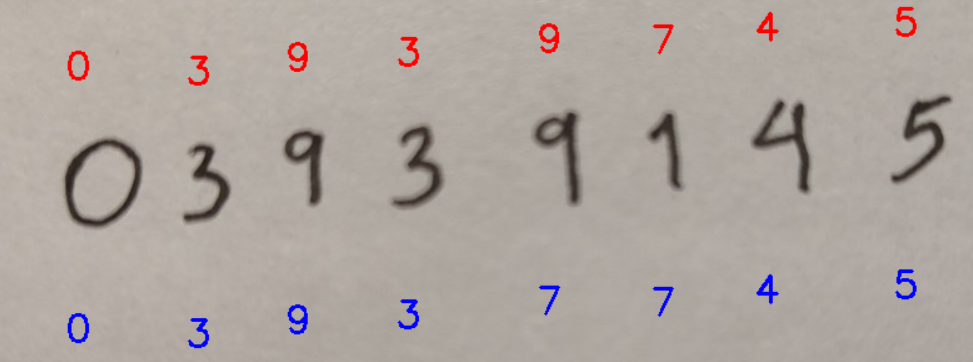
\includegraphics[width=\textwidth]{Image/test1.png}

    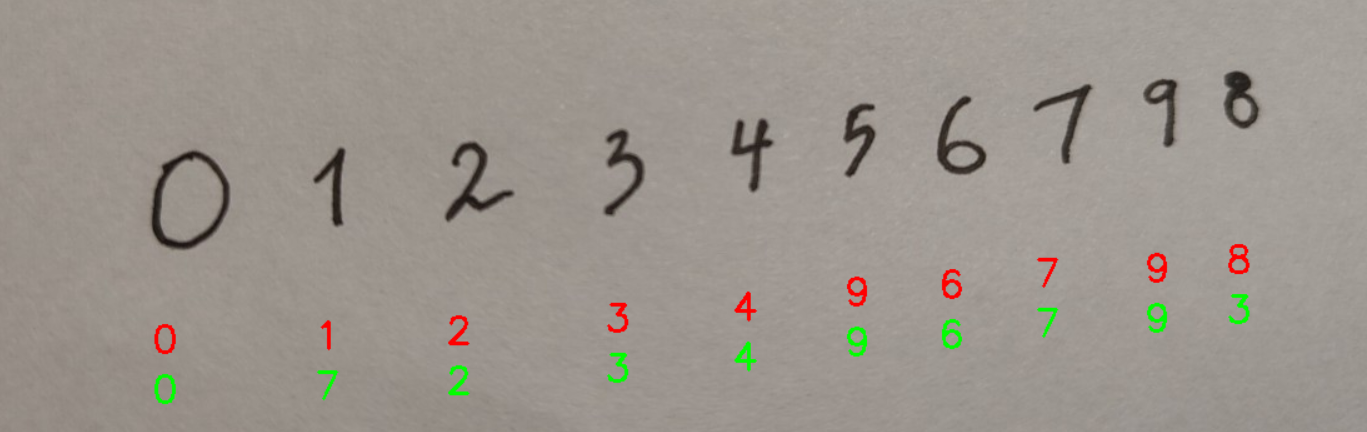
\includegraphics[width=\textwidth]{Image/test2.png}
    \caption{Kết quả dự đoán}
    \label{fig 2.8:Kết quả dự đoán}
\end{figure}

Từ hình 2.8 ta thấy. Ở bức ảnh phía trên, khi các chữ số được viết khá rõ ràng thì cả hai mô hình đều đưa ra dự đoán sai 1 chữ số.
Tuy nhiên ở hình dưới, khi các chữ số bị viết xấu hơn, các nét viết nguệch ngoạc thì mô hình Adversarial-regularized chỉ dự đoán sai 1/10 chữ số, trong khi mô hình cơ bản dự đoán sai 3/10 chữ số.
Từ đó ta thấy rằng, mô hình Adversarial-regularized có độ chính xác cao hơn và hoạt động tốt hơn mô hình cơ bản khi dữ liệu bị nhiễu. Và đây là một trong những ưu điểm của mô hình Adversarial-regularized.


%
\chapter{Kết luận} % Tên của chương

\label{Chapter3} % Thay X bằng số chương tương ứng; để trích dẫn chương này ở chỗ nào đó trong bài, hãy sử dụng lệnh \ref{ChapterX} 

Qua các chương trên chúng ta đã có cái nhìn tổng quan về TensorFlow, Neural Structured Learning. Chúng ta đã cài đặt và sử dụng  Neural Structured Learning
để xử lý bài toán phân loại chữ số viết tay. Chúng ta biết rằng Neural Structured Learning được khái quát hóa bằng hai phần chính là Neural Graph Learning và
Adversarial Learning tuy nhiên ở chương 2 chúng ta mới chỉ sử dụng Adversarial Learning để thử nghiệm, quan sát và đánh giá nó. Và ở mục 2.2 chúng ta đã minh chứng 
rằng Neural Structured Learning có thể giúp cải thiện độ chính xác của mô hình và giúp các mô hình hoạt động tốt hơn trên những tập dữ liệu kém.

Ở mục 1.1.2 chúng ta thấy rằng chỉ cần thêm một nhiễu rất nhỏ mà mắt thường không thể phát hiện được, ngay lập tức đã đánh lừa được mô hình cơ bản phán đoán sai.
Điều này mang lại nhiều nguy cơ cho các hệ thống sử dụng mạng neural để phát hiện, phân loại hình ảnh như camera an ninh hay xe tự lái vì chỉ cần các bức ảnh mà camera
thu thập được không đủ tốt hoặc có nhiễu thì sẽ gây ra sai lầm cho các phán đoán cho hệ thống. Đặc biệt là một số kẻ xấu có thể lợi dụng điều này để tấn công vào các hệ thống an ninh sử dụng
camera và thực hiện các hành vi của mình. Vì vậy việc tìm ra các cách để cải thiện độ chính xác của mô hình trên các tập dữ liệu kém tương tự như Adversarial Learning là rất cần thiết. 
%\include{Chapters/Chapter5} 


%----------------------------------------------------------------------------------------
%	Phần 15: PHỤ LỤC (THESIS CONTENT - APPENDICES)
%----------------------------------------------------------------------------------------

\appendix % Nói với LaTeX rằng những chương về sau được tính là phụ lục

% Hãy thêm những phụ lục (appendix) của khóa luận/tiểu luận vào thư mục Appendices
% Hãy bỏ chú thích những dòng nếu bạn đã bổ sung những phụ lục vào

% Phụ lục A

\chapter{Các câu hỏi thường gặp} % Tên của phụ lục

\label{AppendixA} % Để trích dẫn chương này ở chỗ nào đó trong bài, hãy sử dụng lệnh \ref{AppendixA} 

%----------------------------------------------------------------------------------------

\section{Làm sao để thay đổi màu của đường dẫn liên kết?}

Màu sắc của đường dẫn có thể được thay đổi bằng các lệnh sau:

{\small\verb!\hypersetup{urlcolor=red}!}, hoặc

{\small\verb!\hypersetup{citecolor=green}!}, hoặc

{\small\verb!\hypersetup{allcolor=blue}!}.

\noindent Nếu bạn muốn ẩn toàn bộ đường dẫn, bạn có thể dùng lệnh:

{\small\verb!\hypersetup{allcolors=.}!}, hoặc thậm chí tốt hơn: 

{\small\verb!\hypersetup{hidelinks}!}.

\noindent Nếu bạn muốn hiển thị đường dẫn có màu trên file PDF còn ở bản in ra thì không, hãy sử dụng:

{\small\verb!\hypersetup{colorlinks=false}!}.


%----------------------------------------------------------------------------------------

\section{Làm sao để biểu diễn một bảng số liệu dài (hơn 1 trang), hoặc một bảng quá to?}

Thay vì sử dụng lệnh {\small\verb!\begin{table}!}, bạn hãy sử dụng lệnh {\small\verb!\begin{longtable}!}. Gói bổ trợ \code{longtable} (đã có sẵn trong template này) sẽ tự động giúp bạn ngắt bảng tại một vị trí khi bảng đã quá dài và biểu diễn phần còn lại của bảng ở những trang tiếp theo. Tài liệu về \code{longtable} bạn có thể tham khảo tại \href{https://mirror.kku.ac.th/CTAN/macros/latex/required/tools/longtable.pdf}{đường dẫn này}.

Trong trường hợp bảng số liệu dài theo bề ngang, bạn có thể xem xét phương án biểu diễn bảng số liệu theo chiều ngang của trang giấy như ví dụ Bảng~\ref{tab:treatments2} dưới đây. Để thực hiện cách này, bạn khai báo bảng như bình thường, rồi thay lệnh {\small\verb!\begin{table}!} bằng lệnh {\small\verb!\begin{sidewaystable}!}. Gói bổ trợ cho lệnh này đã có sẵn trong template này.

\begin{sidewaystable}
	\caption{Ảnh hưởng của phương pháp điều trị X và Y đối với bốn nhóm được nghiên cứu.}
	\label{tab:treatments2}
	\centering
	\begin{tabular}{l l l}
		\toprule
		\tabhead{Nhóm} & \tabhead{Phương pháp X} & \tabhead{Phương pháp Y} \\
		\midrule
		1	& 0.20	& 0.80	\\
		2	& 0.17	& 0.70	\\
		3	& 0.24	& 0.75	\\
		4	& 0.68	& 0.30	\\
		\bottomrule	\\
	\end{tabular}
\end{sidewaystable}


%----------------------------------------------------------------------------------------

\section{Làm sao để tìm đoạn code dưới định dạng bibtex cho tài liệu trích dẫn một cách hiệu quả?}

Bạn có thể tham khảo một số cách sau đây:

\begin{itemize}
	\item Cách 1: Sử dụng trang \href{https://scholar.google.com}{scholar.google.com}\\
	Bạn sẽ cần đi đến trang \href{https://scholar.google.com}{scholar.google.com} và hãy dán chính xác tên bài báo bạn muốn tìm kiếm. Sau đó bạn sẽ thấy một danh sách rất nhiều các đường dẫn đến bài báo và cả các bài báo tương tự mà bạn tìm kiếm. Hãy click vào biểu tượng: \textcolor{blue}{\faQuoteRight\;Cite}, rồi chọn tùy chọn \option{BibTeX} và bạn sẽ thấy đoạn code bạn cần.
	\item Cách 2: Sử dụng trang \href{https://www.researchgate.net/search}{researchgate.net}\\
	Bạn sẽ cần đi đến trang \href{https://www.researchgate.net/search}{researchgate.net} và hãy dán chính xác tên bài báo bạn muốn tìm kiếm. Sau đó bạn sẽ thấy một danh sách rất nhiều các đường dẫn đến bài báo và cả các bài báo tương tự mà bạn tìm kiếm. Hãy click vào tên bài báo phù hợp, sau đó click vào \option{Download citation}, rồi chọn tùy chọn \option{BibTeX} và \option{Citation only}. Để thuận tiện, bạn không cần download file chứa nội dung BibTeX về mà chỉ đơn giản chọn \option{Copy to clipboard} rồi dán nội dung vừa copy vào file \file{main.bib} của mình.
	\item Cách 3: Nếu một số tài liệu không xuất hiện ở cả hai trang phía trên, những tài liệu này thường là phần mềm hoặc kỉ yếu hoặc sách. Đối với phần mềm hoặc kỉ yếu, bạn có thể đi đến trang web chính thức chứa phần mềm hoặc kỉ yếu đó, nhiều khả năng là trang web sẽ hỗ trợ bạn trong việc trích dẫn. Đối với sách, bạn có nên tự xây dựng đoạn code BibTeX dựa trên một số đoạn code tương tự rồi thay đổi nội dung như số chương, số trang bạn đang muốn trích dẫn tới sao cho phù hợp.
\end{itemize}







% Phụ lục B

\chapter{Liệt kê source code} % Tên của phụ lục

\label{AppendixB} % Để trích dẫn chương này ở chỗ nào đó trong bài, hãy sử dụng lệnh \ref{AppendixB} 

%----------------------------------------------------------------------------------------

\section{Ví dụ liệt kê code ngôn ngữ C/C++}

Code tính khoảng thời gian giữa hai thời điểm cho trước. Lệnh thực hiện là:
\begin{Verbatim}
\lstinputlisting{"Code/TimeDiff.cpp"}
\end{Verbatim}

File \file{TimeDiff.cpp}:
%https://www.programiz.com/cpp-programming/examples/time-structure
\lstinputlisting{"Code/TimeDiff.cpp"}


%----------------------------------------------------------------------------------------

\section{Ví dụ liệt kê thông tin ở terminal (console/command prompt) từ file text}

Sau khi biên dịch và chạy file \file{TimeDiff.cpp}, kết quả chạy được hiển thị ở terminal. Trong trường hợp bạn muốn liệt kê quá trình chạy, bạn có thể copy đoạn text ở terminal vào một file text, và liệt kê chúng chẳng hạn như:
\begin{Verbatim}
\lstinputlisting[style=console]{"Code/TimeDiff.txt"}
\end{Verbatim}

File \file{TimeDiff.txt}:
\lstinputlisting[style=console]{"Code/TimeDiff.txt"}


%----------------------------------------------------------------------------------------

\section{Ví dụ liệt kê code ngôn ngữ Python}

Code tính mã hash của một file. Lệnh thực hiện là:
\begin{Verbatim}
\lstinputlisting[style=codePython]{"Code/Hash.py"}
\end{Verbatim}

File \file{Hash.py}:
%https://www.programiz.com/python-programming/examples/hash-file
\lstinputlisting[style=codePython]{"Code/Hash.py"}


%----------------------------------------------------------------------------------------

\section{Ví dụ liệt kê code ngôn ngữ Matlab}

Code biểu diễn bản chất và sai số của phương pháp Euler và Heun trong việc giải phương trình vi phân. Lệnh thực hiện là:
\begin{Verbatim}
\lstinputlisting[style=codeMatlab]{"Code/EulerVisualization.m"}
\end{Verbatim}

File \file{EulerVisualization.m}:
\lstinputlisting[style=codeMatlab]{"Code/EulerVisualization.m"}


%----------------------------------------------------------------------------------------

\section{Ví dụ liệt kê file text thông thường (plain text)}

Một file text lưu giữ thông số của một lần chạy mô phỏng động học phân tử. Lệnh thực hiện là:
\begin{Verbatim}
\lstinputlisting[style=plaintext]{"Code/minim.mdp"}
\end{Verbatim}

File \file{minim.mdp}:
\lstinputlisting[style=plaintext]{"Code/minim.mdp"}




%\include{Appendices/AppendixC}


%----------------------------------------------------------------------------------------
%	(KHÔNG CHỈNH SỬA PHẦN NÀY)
%
%	Phần 16: TÀI LIỆU THAM KHẢO
%----------------------------------------------------------------------------------------

\begin{spacing}{1.15}
	\printbibliography[heading=bibintoc, title=Tài liệu tham khảo] % In ra tài liệu tham khảo
\end{spacing}

%----------------------------------------------------------------------------------------

\end{document}  
